% Options for packages loaded elsewhere
\PassOptionsToPackage{unicode}{hyperref}
\PassOptionsToPackage{hyphens}{url}
%
\documentclass[
]{article}
\usepackage{lmodern}
\usepackage{amssymb,amsmath}
\usepackage{ifxetex,ifluatex}
\ifnum 0\ifxetex 1\fi\ifluatex 1\fi=0 % if pdftex
  \usepackage[T1]{fontenc}
  \usepackage[utf8]{inputenc}
  \usepackage{textcomp} % provide euro and other symbols
\else % if luatex or xetex
  \usepackage{unicode-math}
  \defaultfontfeatures{Scale=MatchLowercase}
  \defaultfontfeatures[\rmfamily]{Ligatures=TeX,Scale=1}
\fi
% Use upquote if available, for straight quotes in verbatim environments
\IfFileExists{upquote.sty}{\usepackage{upquote}}{}
\IfFileExists{microtype.sty}{% use microtype if available
  \usepackage[]{microtype}
  \UseMicrotypeSet[protrusion]{basicmath} % disable protrusion for tt fonts
}{}
\makeatletter
\@ifundefined{KOMAClassName}{% if non-KOMA class
  \IfFileExists{parskip.sty}{%
    \usepackage{parskip}
  }{% else
    \setlength{\parindent}{0pt}
    \setlength{\parskip}{6pt plus 2pt minus 1pt}}
}{% if KOMA class
  \KOMAoptions{parskip=half}}
\makeatother
\usepackage{xcolor}
\IfFileExists{xurl.sty}{\usepackage{xurl}}{} % add URL line breaks if available
\IfFileExists{bookmark.sty}{\usepackage{bookmark}}{\usepackage{hyperref}}
\hypersetup{
  pdftitle={DATA 621 - Final Paper},
  pdfauthor={Abdelmalek Hajjam/ Monu Chacko},
  hidelinks,
  pdfcreator={LaTeX via pandoc}}
\urlstyle{same} % disable monospaced font for URLs
\usepackage[margin=1in]{geometry}
\usepackage{color}
\usepackage{fancyvrb}
\newcommand{\VerbBar}{|}
\newcommand{\VERB}{\Verb[commandchars=\\\{\}]}
\DefineVerbatimEnvironment{Highlighting}{Verbatim}{commandchars=\\\{\}}
% Add ',fontsize=\small' for more characters per line
\usepackage{framed}
\definecolor{shadecolor}{RGB}{248,248,248}
\newenvironment{Shaded}{\begin{snugshade}}{\end{snugshade}}
\newcommand{\AlertTok}[1]{\textcolor[rgb]{0.94,0.16,0.16}{#1}}
\newcommand{\AnnotationTok}[1]{\textcolor[rgb]{0.56,0.35,0.01}{\textbf{\textit{#1}}}}
\newcommand{\AttributeTok}[1]{\textcolor[rgb]{0.77,0.63,0.00}{#1}}
\newcommand{\BaseNTok}[1]{\textcolor[rgb]{0.00,0.00,0.81}{#1}}
\newcommand{\BuiltInTok}[1]{#1}
\newcommand{\CharTok}[1]{\textcolor[rgb]{0.31,0.60,0.02}{#1}}
\newcommand{\CommentTok}[1]{\textcolor[rgb]{0.56,0.35,0.01}{\textit{#1}}}
\newcommand{\CommentVarTok}[1]{\textcolor[rgb]{0.56,0.35,0.01}{\textbf{\textit{#1}}}}
\newcommand{\ConstantTok}[1]{\textcolor[rgb]{0.00,0.00,0.00}{#1}}
\newcommand{\ControlFlowTok}[1]{\textcolor[rgb]{0.13,0.29,0.53}{\textbf{#1}}}
\newcommand{\DataTypeTok}[1]{\textcolor[rgb]{0.13,0.29,0.53}{#1}}
\newcommand{\DecValTok}[1]{\textcolor[rgb]{0.00,0.00,0.81}{#1}}
\newcommand{\DocumentationTok}[1]{\textcolor[rgb]{0.56,0.35,0.01}{\textbf{\textit{#1}}}}
\newcommand{\ErrorTok}[1]{\textcolor[rgb]{0.64,0.00,0.00}{\textbf{#1}}}
\newcommand{\ExtensionTok}[1]{#1}
\newcommand{\FloatTok}[1]{\textcolor[rgb]{0.00,0.00,0.81}{#1}}
\newcommand{\FunctionTok}[1]{\textcolor[rgb]{0.00,0.00,0.00}{#1}}
\newcommand{\ImportTok}[1]{#1}
\newcommand{\InformationTok}[1]{\textcolor[rgb]{0.56,0.35,0.01}{\textbf{\textit{#1}}}}
\newcommand{\KeywordTok}[1]{\textcolor[rgb]{0.13,0.29,0.53}{\textbf{#1}}}
\newcommand{\NormalTok}[1]{#1}
\newcommand{\OperatorTok}[1]{\textcolor[rgb]{0.81,0.36,0.00}{\textbf{#1}}}
\newcommand{\OtherTok}[1]{\textcolor[rgb]{0.56,0.35,0.01}{#1}}
\newcommand{\PreprocessorTok}[1]{\textcolor[rgb]{0.56,0.35,0.01}{\textit{#1}}}
\newcommand{\RegionMarkerTok}[1]{#1}
\newcommand{\SpecialCharTok}[1]{\textcolor[rgb]{0.00,0.00,0.00}{#1}}
\newcommand{\SpecialStringTok}[1]{\textcolor[rgb]{0.31,0.60,0.02}{#1}}
\newcommand{\StringTok}[1]{\textcolor[rgb]{0.31,0.60,0.02}{#1}}
\newcommand{\VariableTok}[1]{\textcolor[rgb]{0.00,0.00,0.00}{#1}}
\newcommand{\VerbatimStringTok}[1]{\textcolor[rgb]{0.31,0.60,0.02}{#1}}
\newcommand{\WarningTok}[1]{\textcolor[rgb]{0.56,0.35,0.01}{\textbf{\textit{#1}}}}
\usepackage{longtable,booktabs}
% Correct order of tables after \paragraph or \subparagraph
\usepackage{etoolbox}
\makeatletter
\patchcmd\longtable{\par}{\if@noskipsec\mbox{}\fi\par}{}{}
\makeatother
% Allow footnotes in longtable head/foot
\IfFileExists{footnotehyper.sty}{\usepackage{footnotehyper}}{\usepackage{footnote}}
\makesavenoteenv{longtable}
\usepackage{graphicx,grffile}
\makeatletter
\def\maxwidth{\ifdim\Gin@nat@width>\linewidth\linewidth\else\Gin@nat@width\fi}
\def\maxheight{\ifdim\Gin@nat@height>\textheight\textheight\else\Gin@nat@height\fi}
\makeatother
% Scale images if necessary, so that they will not overflow the page
% margins by default, and it is still possible to overwrite the defaults
% using explicit options in \includegraphics[width, height, ...]{}
\setkeys{Gin}{width=\maxwidth,height=\maxheight,keepaspectratio}
% Set default figure placement to htbp
\makeatletter
\def\fps@figure{htbp}
\makeatother
\setlength{\emergencystretch}{3em} % prevent overfull lines
\providecommand{\tightlist}{%
  \setlength{\itemsep}{0pt}\setlength{\parskip}{0pt}}
\setcounter{secnumdepth}{-\maxdimen} % remove section numbering

\title{DATA 621 - Final Paper}
\author{Abdelmalek Hajjam/ Monu Chacko}
\date{5/22/2020}

\begin{document}
\maketitle

\begin{quote}
``The best investment on earth is earth.'' \textbf{-Louis Glickman}
\end{quote}

\hypertarget{abstract}{%
\section{Abstract}\label{abstract}}

The real estate market in an important aspect in people life. From the
dream of owning a home to using it as a security during tough times,
real estate has been a part of our lives from generations. Price of real
estate is important when buying home. For example, if we are buying
house as an investment they we would want to buy when the prices are
low.

So how exactly are real estate prices determined? Understanding what
factors drive sale prices is both interesting and important. In this
project we use the popular Iowa housing data set to investigate which
factors influence the final sale price. There were many features that we
used when considering this research. Amoung those were location,
condition, size etc.

\hypertarget{key-words}{%
\section{Key Words}\label{key-words}}

Real Estate, Investment Home, Home Prices, Assessed Value, Regression,
Linear Models

\hypertarget{introduction}{%
\section{Introduction}\label{introduction}}

Real estate is property consisting of land and the buildings on it,
along with its natural resources such as crops, minerals or water.
Residential real estate may contain either a single family or
multifamily structure that is available for occupation or for
non-business purposes. Residences can be classified by and how they are
connected to neighbouring residences and land. Different types of
housing tenure can be used for the same physical type. For example,
connected residences might be owned by a single entity and leased out,
or owned separately with an agreement covering the relationship between
units and common areas and concerns.

Apartment, Multi-family house, Terraced house, Condominium, Cooperative,
Duplex etc are some categories of residential realestate. We found it
interesting to study the real-estate market because this market this is
a dynamic market and there are many factors that has influence over it.
The dataset had many features to work with.

The data set was prepared by Dean De Cock in an effort to create a
real-world data set to test and practice regression methods
{[}@DeCock{]}. It describes the sale of individual residential
properties in Ames, Iowa from 2006 to 2010. Founded in 1864 as a station
stop, Ames has a population of approximately 60,000 people, covers about
24.27 square miles and was ranked ninth on the \emph{Best Places to
Live} list {[}@CNNMoney{]}. The original data came directly from the
Ames Assessor's Office recordkeeping database and included information
for calculation of assessed value using the city's assessment process.
The data is recent, and it covers the period of housing bubble collapse
that led to the sub-prime mortgage crisis. The year 2008 saw one of the
largest housing price drops in history.

There are over 2900 total observations and the data represents attribute
of an individual residential property sold. There are about 80 variables
included that cover a multitude of property attributes. Most variables
describe the physical appearance or features of the property but other
variables provide measures of quality and condition. The data types are
varied and include discrete, continuous, and categorical (both nominal
and ordinal) data.

The data was originally published in the Journal of Statistics Education
(Volume 19, Number 3). The data used for regression was downloaded from
Kaggle.com, which allowed us the opportunity to compete against other
kaggle users to find the best-fitting model for this data {[}@Kaggle{]}.

\hypertarget{literature-review}{%
\section{Literature Review}\label{literature-review}}

The paper from MIT Press, ``The Dynamics of Real Estate Prices''
presents an improved methodology which combines information on repeat
sales of unchanged properties, on repeat sales of improved properties,
and on single sales, all in one joint estimation. Empirical evidence,
based upon a rich sample of transactions on single family houses in a
single neighborhood, indicates the clear advantages of the proposed
methodology, at least in one typical application.

The article ``A Regression Method for Real Estate Price Index
Construction'' explains that the quality differences make estimation of
price indexes for real properties difficult, but these can be largely
avoided by basing an index on sales prices of the same property at
different times. The problem of combining price relatives of repeat
sales of properties to obtain a price index can be converted into a
regression problem, and standard techniques of regression analysis can
be used to estimate the index. This method of estimation is more
efficient than others for combining price relatives in that it utilizes
information about the price index for earlier periods contained in sales
prices in later periods. Standard errors of the estimated index numbers
can be readily computed using the regression method, and it permits
certain effects on the value of real properties to be eliminated from
the index.

The article ``Understanding Recent Trends in House Prices and Home
Ownership'' by Robert J. Shiller looks at a broad array of evidence
concerning the recent boom in home prices, and considers what this means
for future home prices and the economy. It does not appear possible to
explain the boom in terms of fundamentals such as rents or construction
costs. A psychological theory, that represents the boom as taking place
because of a feedback mechanism or social epidemic that encourages a
view of housing as an important investment opportunity, fits the
evidence better.

\hypertarget{methodology}{%
\section{Methodology}\label{methodology}}

\hypertarget{data-description}{%
\subsubsection{Data Description}\label{data-description}}

There are 2,910 observation and 79 independent variables in this
dataset. Out of those 36 are numeric, such as lot area or pool area in
square feet, and 43 are categorical, such as garage type (attached to
home, built-in, carport, etc.) or utilities (gas, sewer, both, etc.).
The data set is split into 1,460 observations comprising the training
set and 1,459 observations representing the testing set.

\hypertarget{data-imputation}{%
\subsubsection{Data Imputation}\label{data-imputation}}

Many real-world datasets may contain missing values for various reasons.
They are often encoded as NaNs, blanks or any other placeholders.
Training a model with a dataset that has a lot of missing values can
drastically impact the machine learning model's quality. Some algorithms
such as scikit-learn estimators assume that all values are numerical and
have and hold meaningful value. One way to handle this problem is to get
rid of the observations that have missing data. However, you will risk
losing data points with valuable information. A better strategy would be
to impute the missing values. In other words, we need to infer those
missing values from the existing part of the data.

\textbf{Three main types of missing data}

\begin{itemize}
\tightlist
\item
  Missing completely at random (MCAR)
\item
  Missing at random (MAR)
\item
  Not missing at random (NMAR)
\end{itemize}

\textbf{Common Imputation Techniques}

\begin{itemize}
\tightlist
\item
  Do Nothing
\item
  Imputation Using (Mean/Median) Values
\item
  Imputation Using (Most Frequent) or (Zero/Constant) Values
\item
  Imputation Using k-NN
\item
  Imputation Using Multivariate Imputation by Chained Equation (MICE)
\item
  Imputation Using Deep Learning (Datawig)
\end{itemize}

Example: Multivariate Imputation by Chained Equation (MICE)

\begin{verbatim}
from impyute.imputation.cs import mice

# start the MICE training
imputed_training=mice(train.values)
\end{verbatim}

Original data set included no complete observations (\emph{see table
3}). However, according to the data dictionary, many of the\texttt{NA}
values have a specific meaning. For example, \texttt{NA} in the
\texttt{PoolQC} variable (pool quality) implies that the property has no
pool. Often this logic carried across multiple variables - for example,
\texttt{NA} in \texttt{GarageQual} (garage quality), \texttt{GarageCond}
(garage condition) and \texttt{GarageType} variables all indicate that
the property has no garage. This type of missing value was replaced with
a new category - \emph{No Pool}, \emph{No Garage} or similar.

After this substitution the number of complete observations increased
significantly to 2,861 or about 98\% of all observations. There remained
only 58 observations with true missing values. These observations
contained 180 missing values in 32 variables. None of the variables
contained a large number of missing values. The top one was
\texttt{MasVnrType} with 24 observations containing \texttt{NA} (0.8\%
of all observations). None of the variables were close to the 5\%
missing threshold that would suggest that we should drop them from
analysis.

In addition to the quantity of missingness being important, why and how
the values are missing can give us insight into whether we have a biased
sample. There are three types of missing data {[}@faraway{]}: 1) Missing
Completely at Random (MCAR), 2) Missing at Random (MAR), and 3) Missing
Not at Random (MNAR). MCAR is when the probability of missingness is the
same for all cases. This is the ideal type of missingness because we
could delete these cases without incurring bias. MAR occurs when the
probability of a value being missing depends upon a known mechanism. In
this scenario, we could delete these observations and compensate by
weighting by group membership. Finally, MNAR occurs when the values are
missing because of an unknown variable. This is the type of missingness
that is most likely to bias our sample. Faraway asserts that
ascertaining the exact nature of the missingness is not possible and
must be inferred. Figure 2 displays the combinations of missing values
in the predictor variables. We may not have MCAR because we can see that
the missingness is not more dispersed across all variables and cases.
Only 32 of the 79 predictors have a missing value, and we notice that
the missingness occurs most often in some of the masonry, basement and
garage variables. There is no indication that values are missing not at
random and given the small number of missing values, we believe the
bias, if any, will be limited.

\hypertarget{data-preparation}{%
\subsubsection{Data Preparation}\label{data-preparation}}

Data preparation is the process of cleaning and transforming raw data
prior to processing and analysis. It is an important step prior to
processing and often involves reformatting data, making corrections to
data and the combining of data sets to enrich data. Data preparation is
often a lengthy undertaking for data professionals or business users,
but it is essential as a prerequisite to put data in context in order to
turn it into insights and eliminate bias resulting from poor data
quality. For example, the data preparation process usually includes
standardizing data formats, enriching source data, and/or removing
outliers.

Categorical variables were inspected and their order was changed to
match the most likely low-to-high order. These variables for the most
part do not rely on the order of categories, so this step was not
critical to modeling; however, it makes the modeling output more
readable and easier to interpret.

As is the case with most data sets, we found several values that were
clearly typos and input errors. For instance, one observation had the
year when garage was built listed as 2207. During data preparation we
noticed some negative values which did not make sense, for example age
etc. They were set to 0.

\hypertarget{data-transformation}{%
\subsubsection{Data Transformation}\label{data-transformation}}

Data transformation is the process of changing the format, structure, or
values of data. For data analytics projects, data may be transformed at
two stages of the data pipeline. Organizations that use on-premises data
warehouses generally use an ETL (extract, transform, load) process, in
which data transformation is the middle step. Today, most organizations
use cloud-based data warehouses, which can scale compute and storage
resources with latency measured in seconds or minutes. The scalability
of the cloud platform lets organizations skip preload transformations
and load raw data into the data warehouse, then transform it at query
time --- a model called ELT ( extract, load, transform).

Processes such as data integration, data migration, data warehousing,
and data wrangling all may involve data transformation. Data
transformation may be constructive (adding, copying, and replicating
data), destructive (deleting fields and records), aesthetic
(standardizing salutations or street names), or structural (renaming,
moving, and combining columns in a database). There are many ETL tools
that automate the process of data transformation. Data analysts, data
engineers, and data scientists also transform data using scripting
languages such as Python or domain-specific languages like SQL.

Prior to modeling, we have extensively analyzed available variables and
took a few approaches to variable transformations. They were meant to
both simplify existing variables and add new variables that may be
helpful in modeling.

Generally, it is more common to think about the age of the house than
the year it was built. Each age related variable was stored in the data
set in two related variables - year built and year sold. Rather than
trying to work with original variables we have converted them to a
single \emph{age} variable. For house age the value was
\(YrSold - YearBuilt\). Similarly the age of the garage and last
remodeling was added to the data set, and the original year variables
were dropped.

Because we are not dealing with a time series data set, we have
converted \texttt{YrSold} and \texttt{MoSold} variables from numeric to
nominal. It is important to catch seasonality, but does not make sense
to regress on these features as continuous variables.

Using the side-by-side box plots in Figure 4, we examined the
categorical variables with more than two values to see if the variable
can be simplified by combining the values into two groups. Our criteria
for this simplification was if the variables' inner quartile ranges of
the response variable distinctly and logically bifurcate. For example,
in \texttt{FireplaceQu} (fireplace quality), \texttt{HeatingQC} (heating
quality) and \texttt{PoolQC} (pool quality), we noticed that the inner
quartiles are bifurcated into two groups that do not overlap: the
highest \emph{Excellent} value and all other lesser quality conditions.
Additional values that are distinct from other values in the same
variables are the \emph{Wood Shingle} value in the roof material
variable (\texttt{RoofMat1}), the above average values in the garage
quality variable (\texttt{GarageQual}), the gas-related values in the
heating variable (\texttt{Heating}), and the \emph{Partial} value in the
sale condition variable (\texttt{SaleCondition}). Consequently, we
transformed these into dummy variables with appropriate names. This
allowed us to preserve some degrees of freedom that would otherwise be
subtracted if each and every one of the original values were turned into
dummy variables.

We examined whether our modeling would benefit from transforming any of
the predictor variables. To do so, we have automated creation of several
different versions of the predictor variables using \texttt{R}. We took
natural logarithms, square roots and squares of the numerical variables,
and then we calculated every possible pairwise interaction between these
transformations, the original numerical variables and categorical
variables. We then calculated all pairwise correlations between the
interactions and the response variable \texttt{SalePrice}. The top
correlations can be seen in table 6, which is sorted in descending order
by R-squared. We observed that there are several correlation values
higher than the highest correlation between the original predictors and
the response, which is \texttt{OverallQual} at 0.79 (\emph{see table
5}). The most promising transformations involved taking the square of
\texttt{OverallQual} and multiplying it by the log-transformed or
square-root-transformed area variables. We added the top five
interactions to our training data set.

We have created several potential training sets to give use flexibility
in training the model. The \textbf{first} of the three training data
sets we created includes only the original variables with the missing
values imputed. In model building and selection this set is referred to
as the \emph{original} data set. The \textbf{second} training data set
includes seven ``simplified'' dummy variables instead of original
variables. It also includes the five highly-correlated interactions.
This set is referred to as the \emph{transformed} data set. The
\textbf{third} training data set includes the same predictor variables
as in the second set with a transformed response variable. While
creating all interactions, we noticed that the correlation values
appeared to increase vis-a-vis the square root of the response variable.
Consequently, since the response variable contains only positive values,
we created a simple BIC step model and used it to calculate the Box-Cox
\(\lambda\) value and transform the response variable. According to
Box-Cox, a \(\lambda\) value of approximately 0.184 should help the
final model meet the normality assumption. This set is referred as the
\emph{Box-Cox} data set.

The effects of this transformation can be see in the scatter plots of
the independent variables on \texttt{SalePrice}. The trends are more
decernable in the transformed data and the relations are generally more
linear (\emph{see figure 6}).

\hypertarget{modeling}{%
\subsubsection{Modeling}\label{modeling}}

Data modeling is the process of producing a descriptive diagram of
relationships between various types of information that are to be stored
in a database. One of the goals of data modeling is to create the most
efficient method of storing information while still providing for
complete access and reporting.

For this research we relied on building and optimizing general linear
model because we are dealing with continuous variable i.e.~house sale
price.

After fitting three baseline models to all three training data sets,
ANOVA demonstrated statistical significance between the original data
set and the transformed data set. While all multiple \(R^2\) values were
within some negligible deviation of each other, adding a Box-Cox
transformation of the response variable improved the \(R^2\) beyond the
model based on the original data set.

We took the strongest model, and applied step-wise regression. Since we
started with the baseline model containing all variables we applied
backward elimination in order to settle on a model with the lowest
Akaike information criterion (AIC) value.

For the variables that were not transformed, we used log-transformation
as it tends to bring sales data closer to normal distribution.

Models used in this research:

\begin{itemize}
\item
  \textbf{Model 1} is based on the fully transformed data set with
  Box-Cox transformed response variable. It includes all available
  predictor variables including any interactions created in data
  preparation. This model explains nearly 94\% of variability of the
  response variable. A good starting point, but we can remove some
  insignificant variables for a more parsimonious model with a decreased
  risk of overfitting.
\item
  \textbf{Model 2} is based on Model 1 modified with step-wise
  regression (backward elimination). It is an improvement with lower
  number of parameters (156 comparing to 237). The multiple \(R^2\)
  value is similar. Comparing two models using ANOVA indicates that they
  are not significantly different.
\item
  \textbf{Model 3} selects only statistically highly significant
  variables from the previous model (p-value is nearly 0). \(R^2\) drops
  and F-statistic rises, so even though the model is simpler with only
  58 parameters, it may not be an improvement. Comparing this model with
  the first one using ANOVA, shows that there is significant difference
  between the two.
\item
  \textbf{Model 4} expands on the previous model by using statistically
  significant variables, but with less strict criteria (p-value
  \textless{} 0.01). The number of parameters is increased, but \(R^2\)
  is also increased. Similarly, per ANOVA, this model is significantly
  different from models 1 and 3.
\item
  \textbf{Model 5} takes variables identified in the previous model, but
  it is trained on the original data set without interactions. It uses
  only log-transformation of \texttt{LotArea} predictor variable and
  \texttt{SalePrice} response variable. This model represents the best
  results based on \(R^2\) for any model we have tried using the
  original data set.
\item
  \textbf{Model 6} is based on Model 4, but it is trained on the
  transformed data set that includes interactions, but not the Box-Cox
  transformation of the response variable. Similarly to model 5, this
  model uses log-transformed \texttt{LotArea} and \texttt{SalePrice}.
\end{itemize}

For all models the F-statistic's p-value shows a drastic improvement
over an intercept-only model, so we can infer that these models are
statistically significant.

The table below summarizes the models. We can see a steady improvement
in AIC numbers for models 1 through 6. Adjusted \(R^2\) fluctuates, but
it remains high, and the values are close between various models. The
fluctuation in \(R^2\) is not enough to be the deciding factor in
selecting a model.

\begin{longtable}[]{@{}lrrrr@{}}
\toprule
\begin{minipage}[b]{0.27\columnwidth}\raggedright
Model\strut
\end{minipage} & \begin{minipage}[b]{0.17\columnwidth}\raggedleft
Multiple R\^{}2\strut
\end{minipage} & \begin{minipage}[b]{0.17\columnwidth}\raggedleft
Adjusted R\^{}2\strut
\end{minipage} & \begin{minipage}[b]{0.09\columnwidth}\raggedleft
AIC\strut
\end{minipage} & \begin{minipage}[b]{0.17\columnwidth}\raggedleft
Kaggle Score\strut
\end{minipage}\tabularnewline
\midrule
\endhead
\begin{minipage}[t]{0.27\columnwidth}\raggedright
Model 1 (Box-Cox)\strut
\end{minipage} & \begin{minipage}[t]{0.17\columnwidth}\raggedleft
0.9359\strut
\end{minipage} & \begin{minipage}[t]{0.17\columnwidth}\raggedleft
0.9241\strut
\end{minipage} & \begin{minipage}[t]{0.09\columnwidth}\raggedleft
-531\strut
\end{minipage} & \begin{minipage}[t]{0.17\columnwidth}\raggedleft
NA\strut
\end{minipage}\tabularnewline
\begin{minipage}[t]{0.27\columnwidth}\raggedright
Model 2 (Box-Cox)\strut
\end{minipage} & \begin{minipage}[t]{0.17\columnwidth}\raggedleft
0.9330\strut
\end{minipage} & \begin{minipage}[t]{0.17\columnwidth}\raggedleft
0.9252\strut
\end{minipage} & \begin{minipage}[t]{0.09\columnwidth}\raggedleft
-617\strut
\end{minipage} & \begin{minipage}[t]{0.17\columnwidth}\raggedleft
NA\strut
\end{minipage}\tabularnewline
\begin{minipage}[t]{0.27\columnwidth}\raggedright
Model 3 (Box-Cox)\strut
\end{minipage} & \begin{minipage}[t]{0.17\columnwidth}\raggedleft
0.8934\strut
\end{minipage} & \begin{minipage}[t]{0.17\columnwidth}\raggedleft
0.8890\strut
\end{minipage} & \begin{minipage}[t]{0.09\columnwidth}\raggedleft
-126\strut
\end{minipage} & \begin{minipage}[t]{0.17\columnwidth}\raggedleft
NA\strut
\end{minipage}\tabularnewline
\begin{minipage}[t]{0.27\columnwidth}\raggedright
Model 4 (Box-Cox)\strut
\end{minipage} & \begin{minipage}[t]{0.17\columnwidth}\raggedleft
0.9193\strut
\end{minipage} & \begin{minipage}[t]{0.17\columnwidth}\raggedleft
0.9131\strut
\end{minipage} & \begin{minipage}[t]{0.09\columnwidth}\raggedleft
-440\strut
\end{minipage} & \begin{minipage}[t]{0.17\columnwidth}\raggedleft
NA\strut
\end{minipage}\tabularnewline
\begin{minipage}[t]{0.27\columnwidth}\raggedright
Model 5 (Original)\strut
\end{minipage} & \begin{minipage}[t]{0.17\columnwidth}\raggedleft
0.8935\strut
\end{minipage} & \begin{minipage}[t]{0.17\columnwidth}\raggedleft
0.8857\strut
\end{minipage} & \begin{minipage}[t]{0.09\columnwidth}\raggedleft
-1604\strut
\end{minipage} & \begin{minipage}[t]{0.17\columnwidth}\raggedleft
0.1475\strut
\end{minipage}\tabularnewline
\begin{minipage}[t]{0.27\columnwidth}\raggedright
Model 6 (Transformed)\strut
\end{minipage} & \begin{minipage}[t]{0.17\columnwidth}\raggedleft
0.9183\strut
\end{minipage} & \begin{minipage}[t]{0.17\columnwidth}\raggedleft
0.9120\strut
\end{minipage} & \begin{minipage}[t]{0.09\columnwidth}\raggedleft
-1982\strut
\end{minipage} & \begin{minipage}[t]{0.17\columnwidth}\raggedleft
0.1385\strut
\end{minipage}\tabularnewline
\bottomrule
\end{longtable}

Since the data set comes from Kaggle, we have an easy way to evaluate
our models by predicting the sale price for the testing set and
submitting our predictions. Kaggle provides a score that lets you judge
the performance of our models. We submitted predictions from models 5
and 6. Model 6 was a clear favorite.

Models 1 through 4 rely on the Box-Cox transformation of the response
variable with \(\lambda\) value of 0.184. Although this may slightly
improve a model, it makes conversion of prediction difficult and
confusing. Log-transformation of the response variable used by models 5
and 6 is significantly easier to implement. As such slight improvement
of the Box-Cox model is not enough to justify added complexity of making
predictions. It is important to consider how the model will be
implemented and simplicity matters.

Model 6 is our primary linear regression model to predict house sale
prices.

The model was tuned using k-fold validation (with 10 folds). It was run
through full diagnostic and four leverage points have been identified.
These observations were removed from the training set as it is very
plausible that the sales data set has some uncharacteristic outliers.

Additionally, two categorical variables - \texttt{Condition2} and
\texttt{Utilities} - were removed from the model because they did not
have enough samples in each category. These variables may be meaningful
for predicting the response variable, but there is not enough
information in our small data set for these variable to train on.

The final model had multiple \(R^2\) of 0.9276, adjusted \(R^2\) of
0.9225, AIC of -2172 and Kaggle score of 0.13376. These are the best
values in all categories.

Figure 1 shows the model diagnostics. There is no discernible pattern
among residuals. The Q-Q plot shows some problems with distribution
tails; however, this is not unexpected with sales data - there are bound
to be some really good and some really bad deals out there. Major
leverage points have been accounted for.

Data preparation and transformation, including response variable
transformation, model building and re-building as well as model
diagnostics resulted in a linear regression model to predict house sale
prices.

\hypertarget{experimentation-and-results}{%
\section{Experimentation and
Results}\label{experimentation-and-results}}

Having developed a model and successfully tested it against available
test data, we can now review the results.

Our model has 98 parameters. The majority of those are dummy variables
created for categorical variables. Table 2 lists all parameters and
corresponding coefficients. Please note that our response variable is
log-transformed, so coefficients will only give a general idea of the
impact on the sale price, and not a specific amount.

Linear regression takes the following form:

\begin{center}
$\hat{y} = \beta_0 + \beta_1 x_1 + ... + \beta_p x_p + \epsilon$
\end{center}

Here, \(\hat{y}\) is the predicted outcome, \(x_1\) through \(x_p\) are
selected parameters, \(\beta_1\) through \(\beta_p\) are corresponding
coefficients, \(\beta_0\) is the intercept and \(\epsilon\) is the error
or noise term. We have too many parameters to efficiently write out our
linear model; however, using the coefficient table we can easily
assemble the final formula if desired. The formula used in \texttt{R} is
as follows:

\begin{Shaded}
\begin{Highlighting}[]
\KeywordTok{log}\NormalTok{(SalePrice) }\OperatorTok{~}\StringTok{ }\NormalTok{OverallCond }\OperatorTok{+}\StringTok{ }\NormalTok{Condition1 }\OperatorTok{+}\StringTok{ }\NormalTok{MSZoning }\OperatorTok{+}\StringTok{ }\NormalTok{X1stFlrSF }\OperatorTok{+}\StringTok{ }\NormalTok{X2ndFlrSF }\OperatorTok{+}\StringTok{ }
\StringTok{  }\NormalTok{LowQualFinSF }\OperatorTok{+}\StringTok{ }\NormalTok{Neighborhood }\OperatorTok{+}\StringTok{ }\NormalTok{KitchenQual }\OperatorTok{+}\StringTok{ }\NormalTok{Fireplaces }\OperatorTok{+}\StringTok{ }\NormalTok{WoodDeckSF }\OperatorTok{+}\StringTok{ }
\StringTok{  }\NormalTok{Functional }\OperatorTok{+}\StringTok{ }\NormalTok{FullBath }\OperatorTok{+}\StringTok{ }\NormalTok{BsmtFullBath }\OperatorTok{+}\StringTok{ }\NormalTok{BsmtFinType1 }\OperatorTok{+}\StringTok{ }\NormalTok{BsmtExposure }\OperatorTok{+}\StringTok{ }\NormalTok{BsmtQual }\OperatorTok{+}
\StringTok{  }\NormalTok{LandSlope }\OperatorTok{+}\StringTok{ }\NormalTok{LandContour }\OperatorTok{+}\StringTok{ }\KeywordTok{log}\NormalTok{(LotArea) }\OperatorTok{+}\StringTok{ }\NormalTok{LotFrontage }\OperatorTok{+}\StringTok{ }\NormalTok{LotConfig }\OperatorTok{+}\StringTok{ }\NormalTok{HouseStyle }\OperatorTok{+}\StringTok{ }
\StringTok{  }\NormalTok{RoofStyle }\OperatorTok{+}\StringTok{ }\NormalTok{MasVnrArea }\OperatorTok{+}\StringTok{ }\NormalTok{ScreenPorch }\OperatorTok{+}\StringTok{ }\NormalTok{House_Age_Yrs }\OperatorTok{+}\StringTok{ }\NormalTok{RoofMatl_WdShngl }\OperatorTok{+}
\StringTok{  }\NormalTok{GarageQual_abv_avg }\OperatorTok{+}\StringTok{ }\NormalTok{OverallQual2_x_GrLivArea }\OperatorTok{+}\StringTok{ }\NormalTok{OverallQual2_x_TotRmsAbvGrd_log }\OperatorTok{+}\StringTok{ }
\StringTok{  }\NormalTok{OverallQual2_x_GarageCars}
\end{Highlighting}
\end{Shaded}

\begin{longtable}[]{@{}llr@{}}
\caption{Linear model parameters and coefficients (sorted by category
and coefficient). (10 records)}\tabularnewline
\toprule
\begin{minipage}[b]{0.15\columnwidth}\raggedright
Category\strut
\end{minipage} & \begin{minipage}[b]{0.39\columnwidth}\raggedright
Details\strut
\end{minipage} & \begin{minipage}[b]{0.18\columnwidth}\raggedleft
Coefficient\strut
\end{minipage}\tabularnewline
\midrule
\endfirsthead
\toprule
\begin{minipage}[b]{0.15\columnwidth}\raggedright
Category\strut
\end{minipage} & \begin{minipage}[b]{0.39\columnwidth}\raggedright
Details\strut
\end{minipage} & \begin{minipage}[b]{0.18\columnwidth}\raggedleft
Coefficient\strut
\end{minipage}\tabularnewline
\midrule
\endhead
\begin{minipage}[t]{0.15\columnwidth}\raggedright
\strut
\end{minipage} & \begin{minipage}[t]{0.39\columnwidth}\raggedright
\strut
\end{minipage} & \begin{minipage}[t]{0.18\columnwidth}\raggedleft
9.736404\strut
\end{minipage}\tabularnewline
\begin{minipage}[t]{0.15\columnwidth}\raggedright
Amenities\strut
\end{minipage} & \begin{minipage}[t]{0.39\columnwidth}\raggedright
Basement exposure - Good\strut
\end{minipage} & \begin{minipage}[t]{0.18\columnwidth}\raggedleft
0.051112\strut
\end{minipage}\tabularnewline
\begin{minipage}[t]{0.15\columnwidth}\raggedright
Amenities\strut
\end{minipage} & \begin{minipage}[t]{0.39\columnwidth}\raggedright
Full bathrooms - Basement\strut
\end{minipage} & \begin{minipage}[t]{0.18\columnwidth}\raggedleft
0.040449\strut
\end{minipage}\tabularnewline
\begin{minipage}[t]{0.15\columnwidth}\raggedright
Amenities\strut
\end{minipage} & \begin{minipage}[t]{0.39\columnwidth}\raggedright
Number of fireplaces\strut
\end{minipage} & \begin{minipage}[t]{0.18\columnwidth}\raggedleft
0.030267\strut
\end{minipage}\tabularnewline
\begin{minipage}[t]{0.15\columnwidth}\raggedright
Amenities\strut
\end{minipage} & \begin{minipage}[t]{0.39\columnwidth}\raggedright
Full bathrooms - Above grade\strut
\end{minipage} & \begin{minipage}[t]{0.18\columnwidth}\raggedleft
0.007889\strut
\end{minipage}\tabularnewline
\begin{minipage}[t]{0.15\columnwidth}\raggedright
Amenities\strut
\end{minipage} & \begin{minipage}[t]{0.39\columnwidth}\raggedright
Basement exposure - Minimum\strut
\end{minipage} & \begin{minipage}[t]{0.18\columnwidth}\raggedleft
0.007124\strut
\end{minipage}\tabularnewline
\begin{minipage}[t]{0.15\columnwidth}\raggedright
Amenities\strut
\end{minipage} & \begin{minipage}[t]{0.39\columnwidth}\raggedright
Size of garage\strut
\end{minipage} & \begin{minipage}[t]{0.18\columnwidth}\raggedleft
0.000961\strut
\end{minipage}\tabularnewline
\begin{minipage}[t]{0.15\columnwidth}\raggedright
Amenities\strut
\end{minipage} & \begin{minipage}[t]{0.39\columnwidth}\raggedright
Basement exposure - None\strut
\end{minipage} & \begin{minipage}[t]{0.18\columnwidth}\raggedleft
-0.000683\strut
\end{minipage}\tabularnewline
\begin{minipage}[t]{0.15\columnwidth}\raggedright
Amenities\strut
\end{minipage} & \begin{minipage}[t]{0.39\columnwidth}\raggedright
Basement exposure - No basement\strut
\end{minipage} & \begin{minipage}[t]{0.18\columnwidth}\raggedleft
NA\strut
\end{minipage}\tabularnewline
\begin{minipage}[t]{0.15\columnwidth}\raggedright
Condition\strut
\end{minipage} & \begin{minipage}[t]{0.39\columnwidth}\raggedright
Normal\strut
\end{minipage} & \begin{minipage}[t]{0.18\columnwidth}\raggedleft
0.079479\strut
\end{minipage}\tabularnewline
\bottomrule
\end{longtable}

The attribute with the most negative effect on the sale price is
severely damaged functionality of the house. Major deductions in
functionality (a step above \emph{Severely Damaged}) is also included in
the top five negative attributes. Interestingly, typical functionality
has one of the most positive influences on the sale price. Clearly and
not surprisingly, general house condition that ranges from
\emph{Typical} to \emph{Salvage Only}, is very important to the final
sale price.

Another attribute that influences the sale price negatively is the
Meadow Village neighborhood. Reviewing Ames, Iowa information, we can
quickly notice that the Meadow Village despite its peaceful name is
actually on the edge of town next to the airport. This would be a less
desirable neighborhood in any town. On the opposite side of town, next
to a golf club and to the Ada Hayden Heritage park and lake, is the
Stone Brooke neighborhood. This is one of the most positive attributes.
Again not surprisingly, the most positive and negative neighborhoods are
on completely opposite sides of town.

Other major negative attributes are lack of finished basement and fair
quality of kitchen. Zoning attributes make up other major positive
attributes.

The model confirms a few attributes that can be considered common sense.
For example, location adjacent to the railroad has a negative influence
on the sale price. However, this only applies to the East-West railroad.
The impact of the North-South railroad is positive. It is important to
note that the East-West railroad cuts through the middle of the town
while the North-South railroad only affects a small portion, and it is
clearly a less used railroad.

Other notable factors are the following:

\begin{itemize}
\tightlist
\item
  House age has a negative influence, but not as great as some other
  attributes.
\item
  Being on a cul-de-sac is the most positive lot location. Inside lot
  has a slightly negative effect, and a lot with streets on 2 sides has
  even more negative coefficient. Finally, a lot with streets on 3 sides
  has the biggest negative impact.
\item
  An unfinished basement generally has a negative impact as does a
  low-quality kitchen.
\item
  The square footage of several characteristics, such as first or second
  floor, wood deck, porch, is not important (but the impact is slightly
  positive).
\item
  1.5 and 2.5 story houses seem to be preferred; however, this variable
  is probably highly dependent on the type of houses available in Ames,
  and it could be representative of some other features.
\end{itemize}

\hypertarget{discussion-and-conclusion}{%
\section{Discussion and Conclusion}\label{discussion-and-conclusion}}

Location and condition seem to be major attributes in house sale prices.
There is seasonality to number of houses sold, especially considering
that Ames is a college town; however, it does not appear to be a major
factor.

The biggest limiting factor of our study is that it is based on one
Midwest town's data. This model may not transfer well to other
locations. After all it is not hard to imagine that the driving factors
in Ames, Iowa are quite different from factors in New York, NY or Los
Angeles, California. It is a helpful starting point, but may not be
widely applicable.

Our research is based exclusively on linear regression. Other methods,
such as Support Vector Machines or Random Forrest, may be able to
achieve much better results. This data set provides a rich opportunity
for research, and it would be beneficial to try other methods for
comparison purposes.

\newpage

\hypertarget{appendix-a.-figures}{%
\section{Appendix A. Figures}\label{appendix-a.-figures}}

\begin{center}
Figure 2. Missing values.
\end{center}

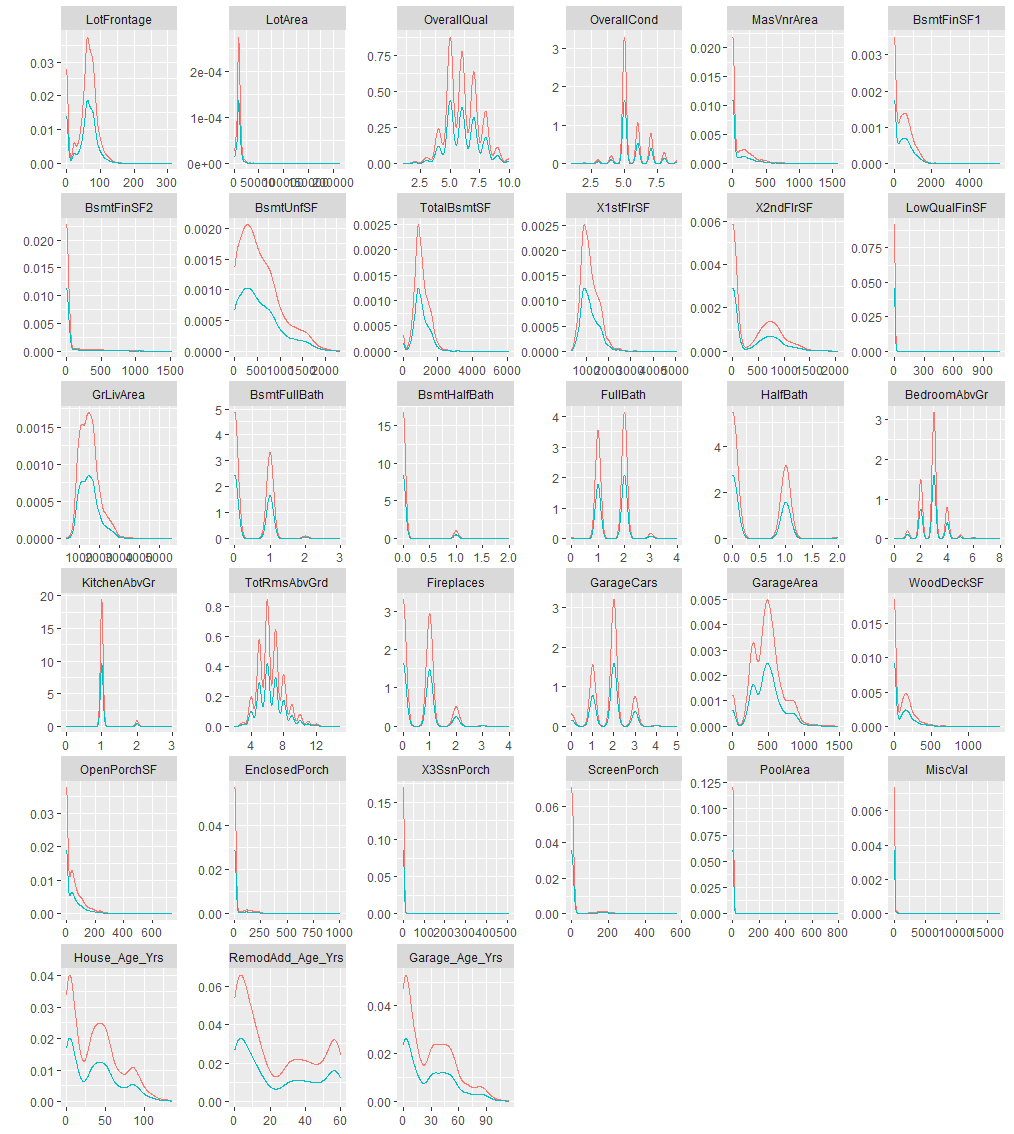
\includegraphics{https://raw.githubusercontent.com/kaiserxc/DATA621FinalProject/master/report_files/fig2_imputation.png}

\begin{center}
Figure 3. Density plots of observed (blue) and imputed (red) values.
\end{center}

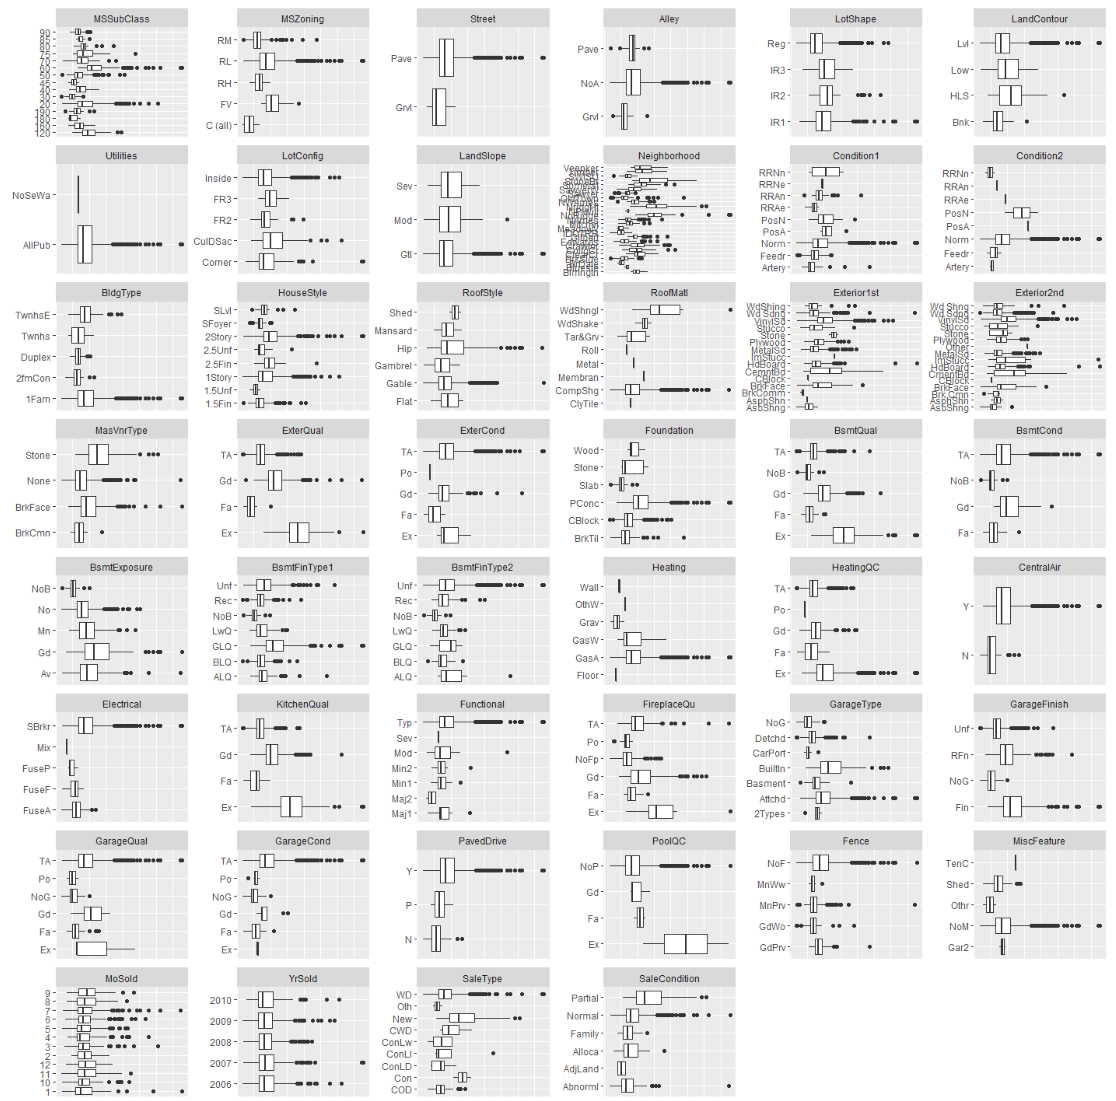
\includegraphics{https://raw.githubusercontent.com/kaiserxc/DATA621FinalProject/master/report_files/fig3_boxplots.png}

\begin{center}
Figure 4. Box plots of categorical variables against the response variable.
\end{center}

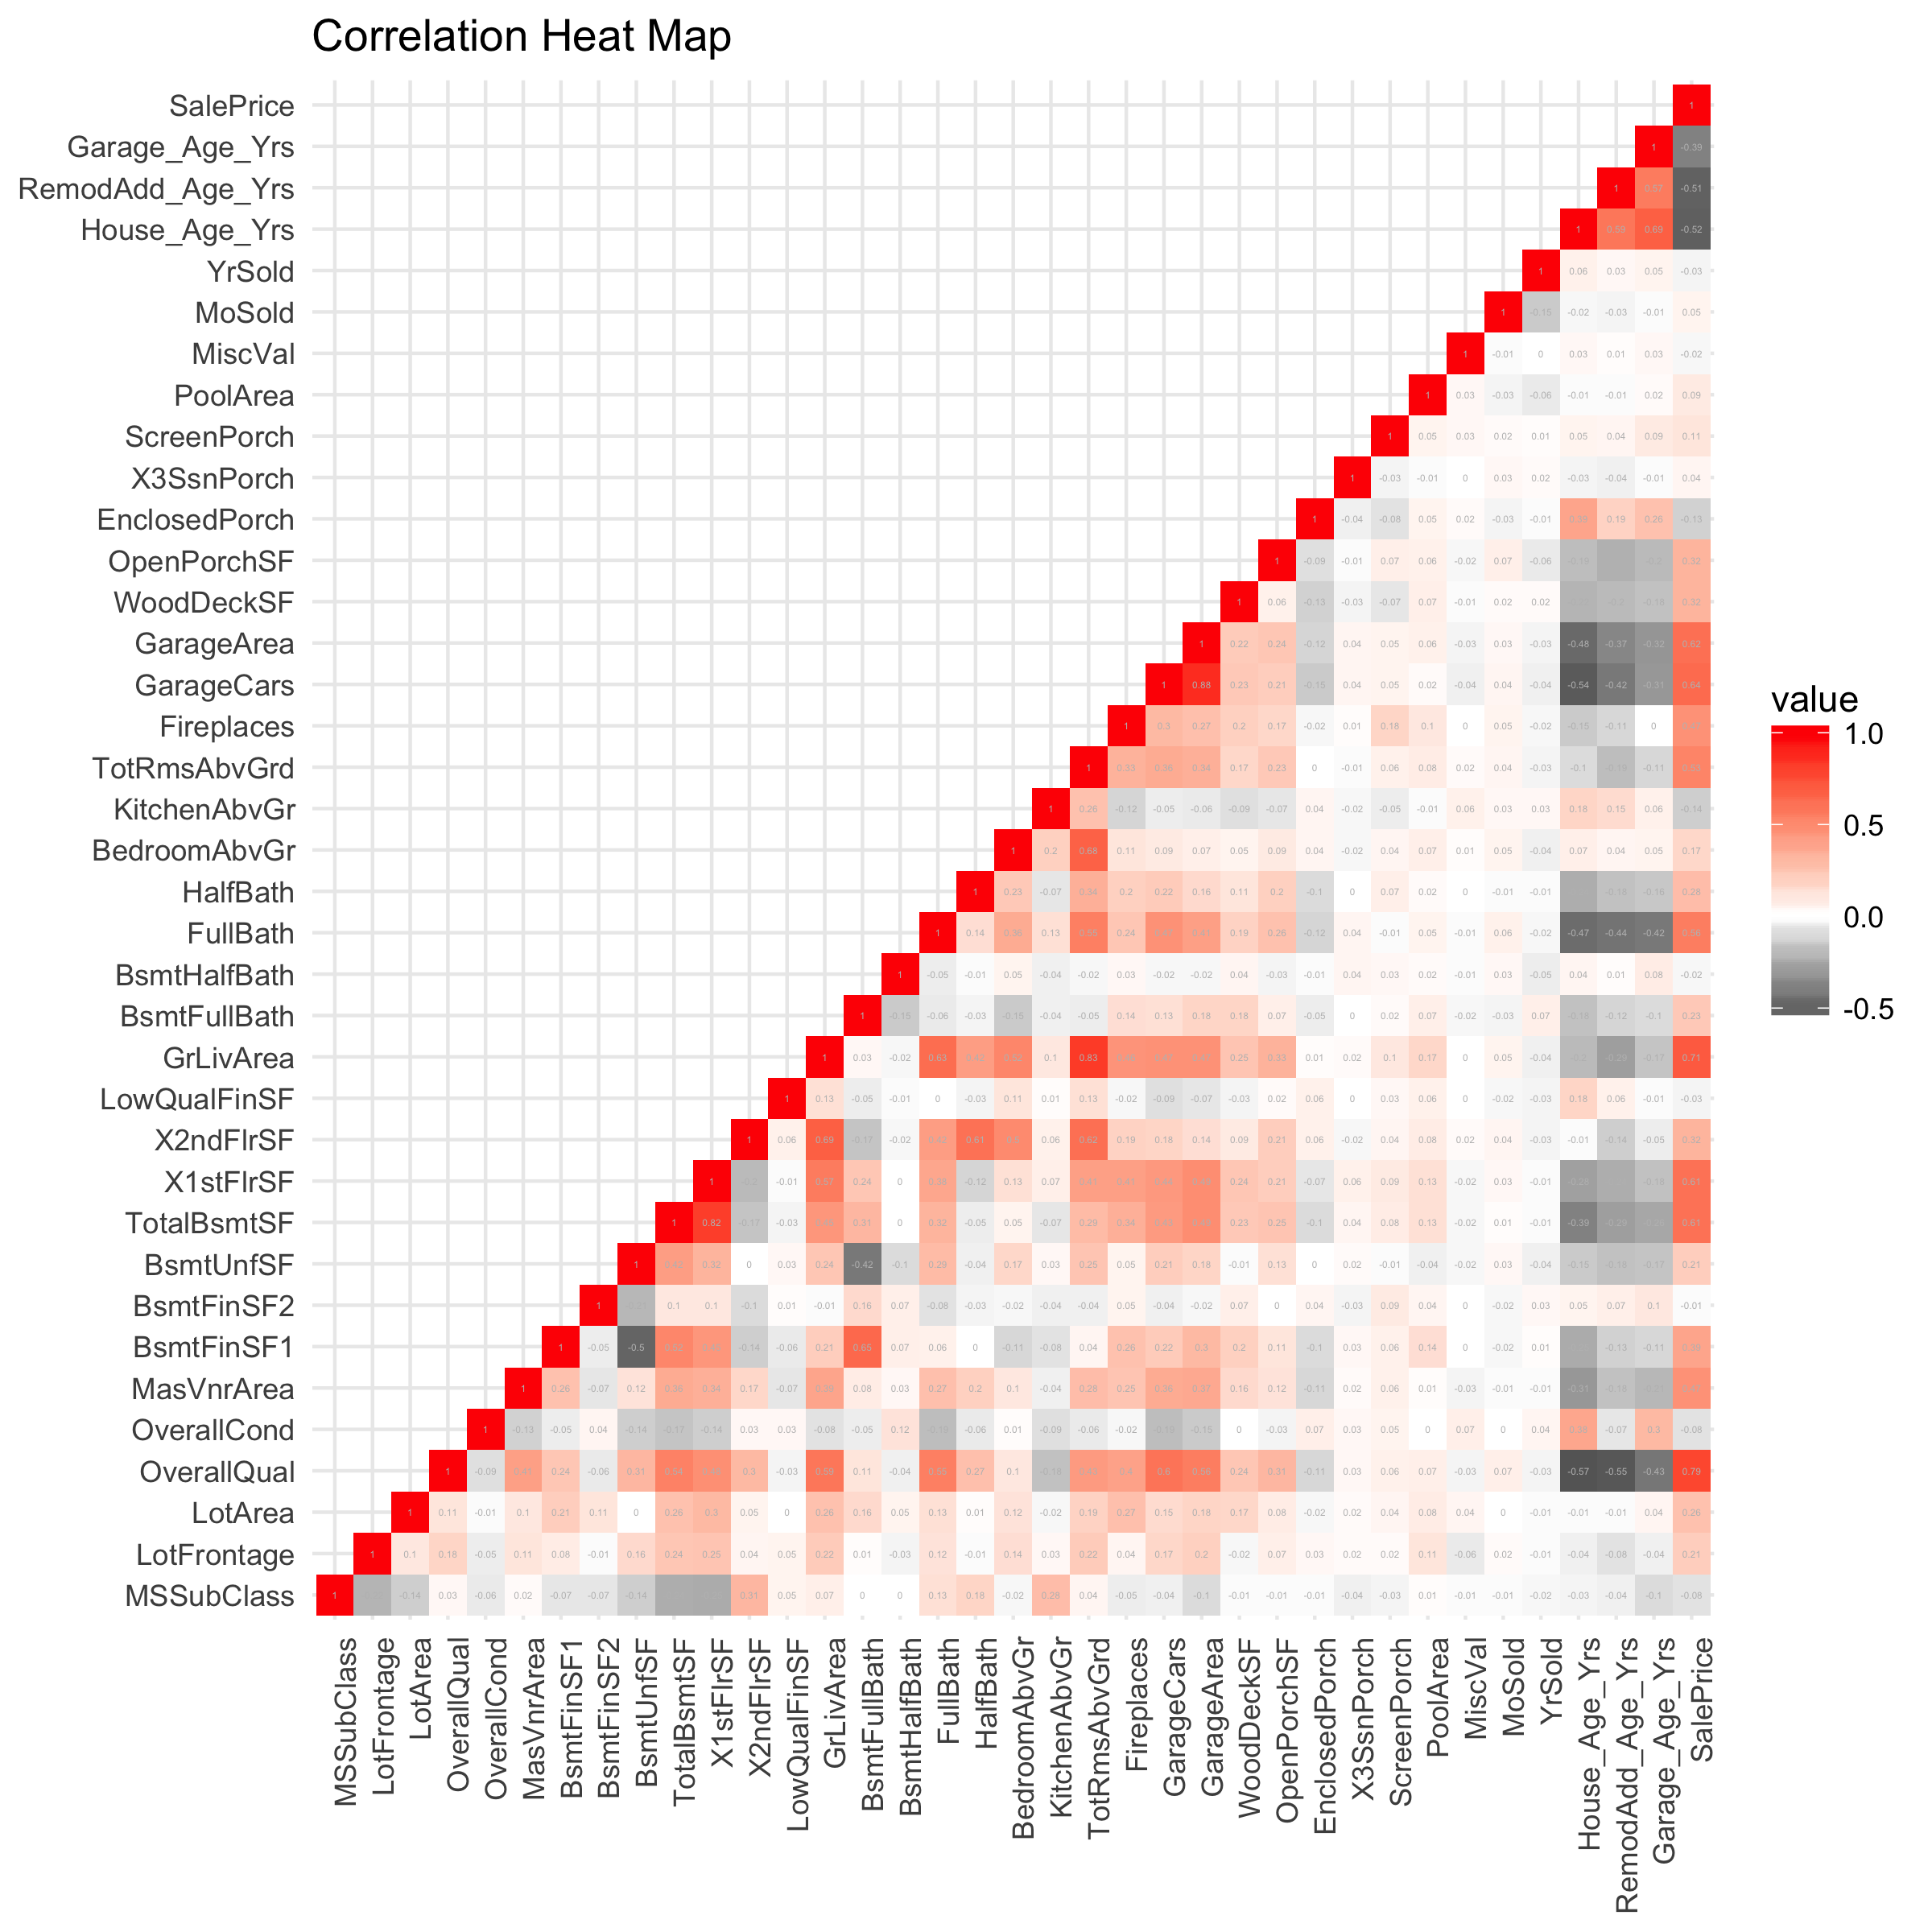
\includegraphics{https://raw.githubusercontent.com/kaiserxc/DATA621FinalProject/master/report_files/fig5_correlation.png}

\begin{center}
Figure 5. Correlation heat map.
\end{center}

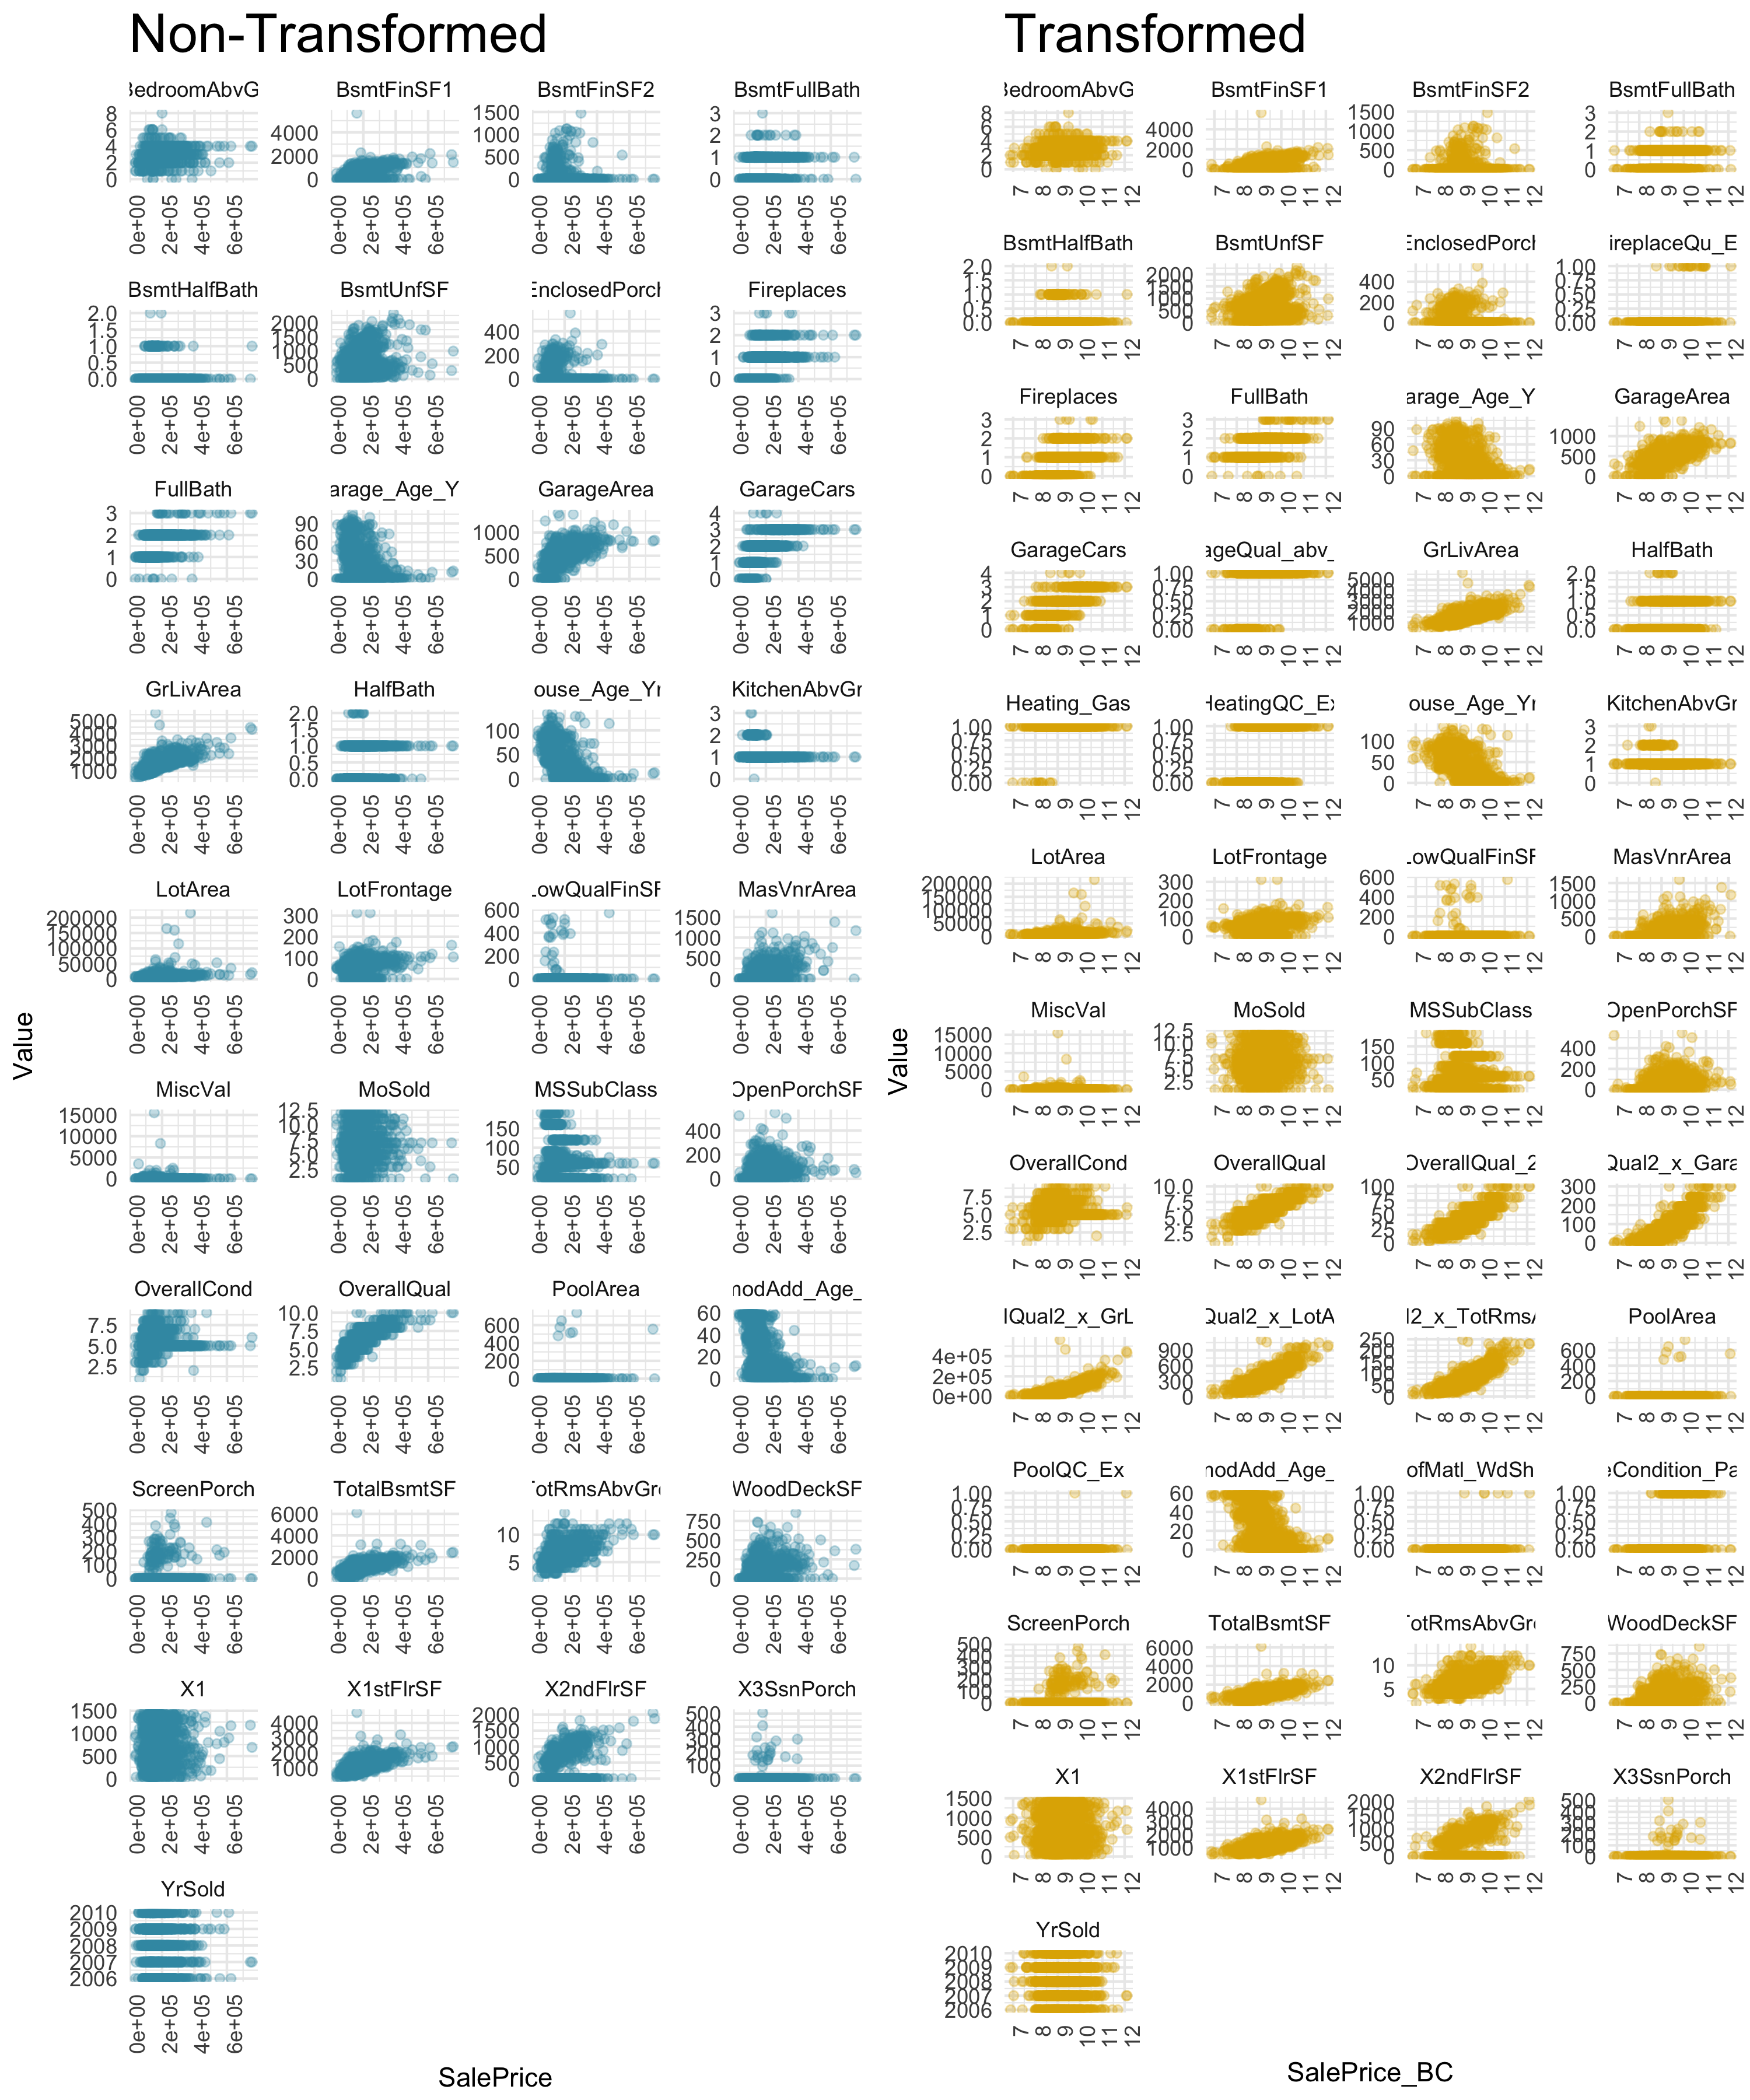
\includegraphics{https://raw.githubusercontent.com/kaiserxc/DATA621FinalProject/master/images/Scatter_Trans_and_Imp.png}

\begin{center}
Figure 6. Scatter plots of original and transformed variables.
\end{center}

\begin{figure}
\centering
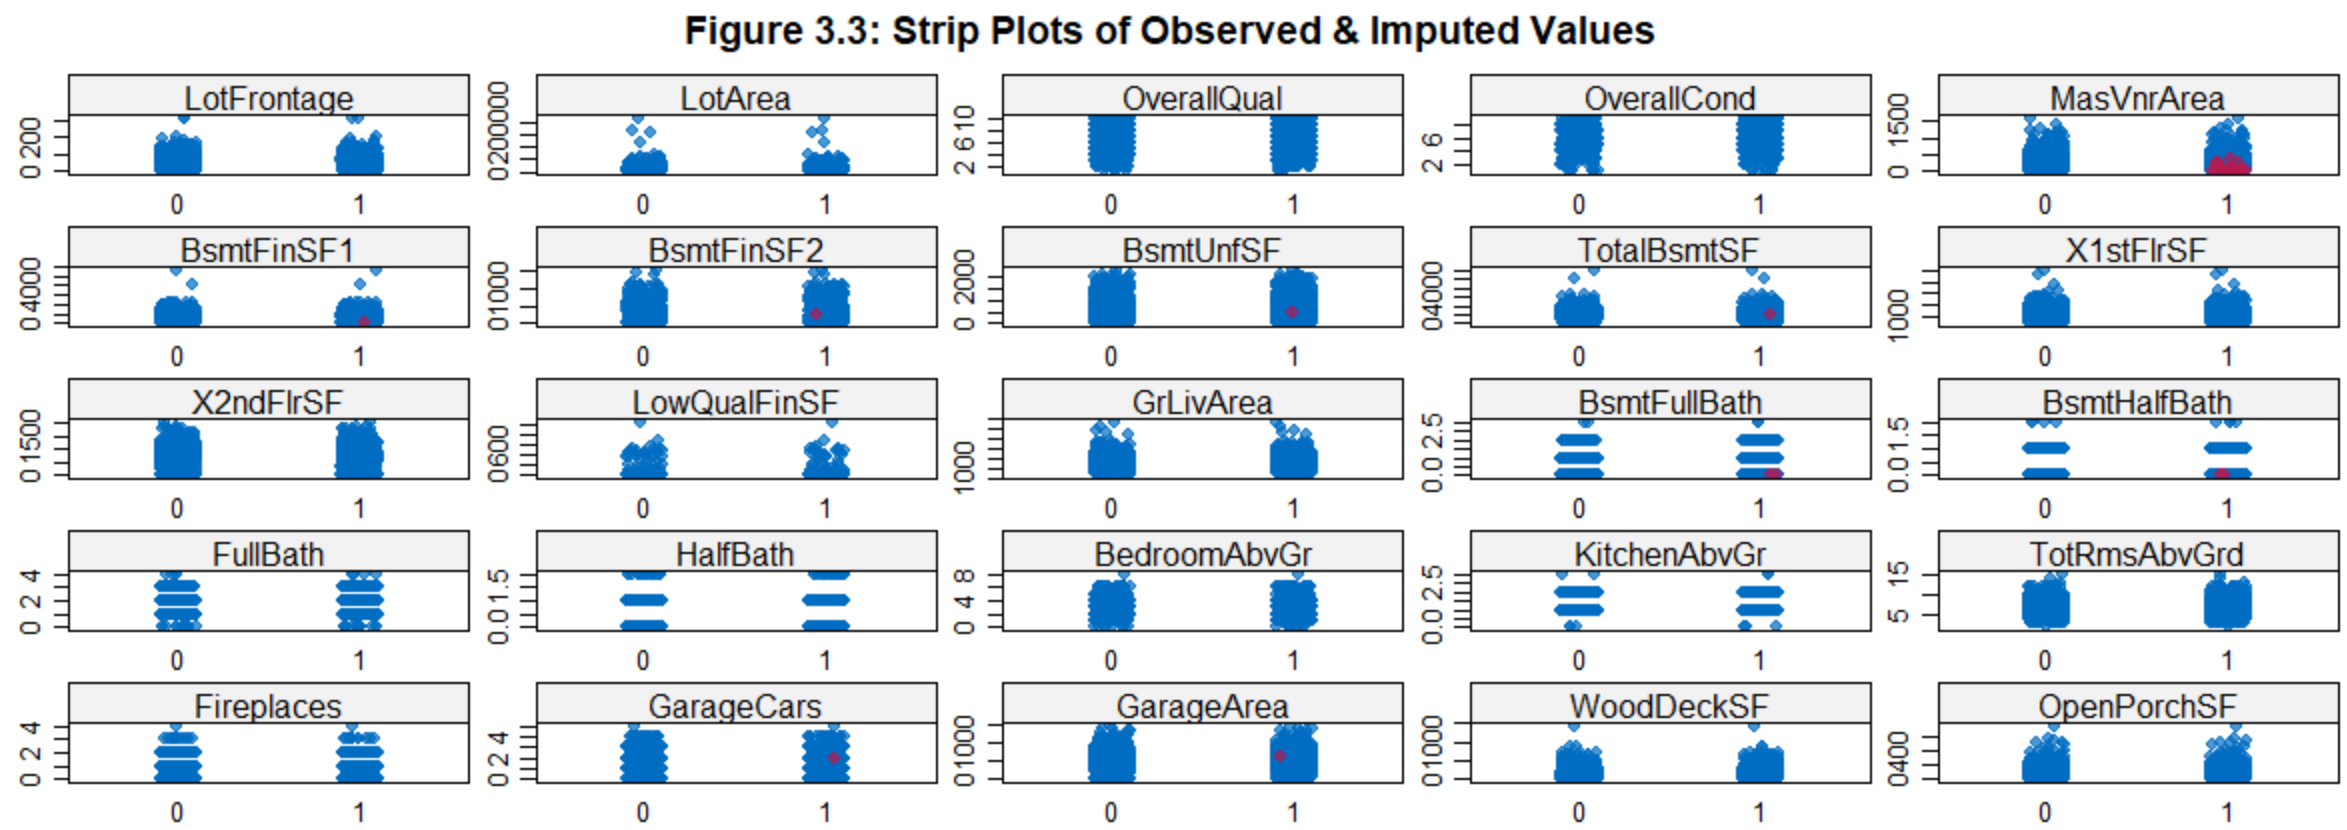
\includegraphics{https://raw.githubusercontent.com/monuchacko/cuny_msds/master/data_621/FinalProject/finalprojectpaper/stripplot_img.png}
\caption{Strip Plots}
\end{figure}

\begin{center}
Figure 6. Scatter plots of original and transformed variables.
\end{center}

\newpage

\hypertarget{appendix-b.-tables}{%
\section{Appendix B. Tables}\label{appendix-b.-tables}}

\begin{longtable}[]{@{}lrr@{}}
\caption{Number of NA values in original data (10
records)}\tabularnewline
\toprule
\begin{minipage}[b]{0.19\columnwidth}\raggedright
Variable\strut
\end{minipage} & \begin{minipage}[b]{0.15\columnwidth}\raggedleft
No of NAs\strut
\end{minipage} & \begin{minipage}[b]{0.29\columnwidth}\raggedleft
Percent of Total Obs\strut
\end{minipage}\tabularnewline
\midrule
\endfirsthead
\toprule
\begin{minipage}[b]{0.19\columnwidth}\raggedright
Variable\strut
\end{minipage} & \begin{minipage}[b]{0.15\columnwidth}\raggedleft
No of NAs\strut
\end{minipage} & \begin{minipage}[b]{0.29\columnwidth}\raggedleft
Percent of Total Obs\strut
\end{minipage}\tabularnewline
\midrule
\endhead
\begin{minipage}[t]{0.19\columnwidth}\raggedright
PoolQC\strut
\end{minipage} & \begin{minipage}[t]{0.15\columnwidth}\raggedleft
2909\strut
\end{minipage} & \begin{minipage}[t]{0.29\columnwidth}\raggedleft
99.66\strut
\end{minipage}\tabularnewline
\begin{minipage}[t]{0.19\columnwidth}\raggedright
MiscFeature\strut
\end{minipage} & \begin{minipage}[t]{0.15\columnwidth}\raggedleft
2814\strut
\end{minipage} & \begin{minipage}[t]{0.29\columnwidth}\raggedleft
96.40\strut
\end{minipage}\tabularnewline
\begin{minipage}[t]{0.19\columnwidth}\raggedright
Alley\strut
\end{minipage} & \begin{minipage}[t]{0.15\columnwidth}\raggedleft
2721\strut
\end{minipage} & \begin{minipage}[t]{0.29\columnwidth}\raggedleft
93.22\strut
\end{minipage}\tabularnewline
\begin{minipage}[t]{0.19\columnwidth}\raggedright
Fence\strut
\end{minipage} & \begin{minipage}[t]{0.15\columnwidth}\raggedleft
2348\strut
\end{minipage} & \begin{minipage}[t]{0.29\columnwidth}\raggedleft
80.44\strut
\end{minipage}\tabularnewline
\begin{minipage}[t]{0.19\columnwidth}\raggedright
FireplaceQu\strut
\end{minipage} & \begin{minipage}[t]{0.15\columnwidth}\raggedleft
1420\strut
\end{minipage} & \begin{minipage}[t]{0.29\columnwidth}\raggedleft
48.65\strut
\end{minipage}\tabularnewline
\begin{minipage}[t]{0.19\columnwidth}\raggedright
LotFrontage\strut
\end{minipage} & \begin{minipage}[t]{0.15\columnwidth}\raggedleft
486\strut
\end{minipage} & \begin{minipage}[t]{0.29\columnwidth}\raggedleft
16.65\strut
\end{minipage}\tabularnewline
\begin{minipage}[t]{0.19\columnwidth}\raggedright
GarageYrBlt\strut
\end{minipage} & \begin{minipage}[t]{0.15\columnwidth}\raggedleft
159\strut
\end{minipage} & \begin{minipage}[t]{0.29\columnwidth}\raggedleft
5.45\strut
\end{minipage}\tabularnewline
\begin{minipage}[t]{0.19\columnwidth}\raggedright
GarageFinish\strut
\end{minipage} & \begin{minipage}[t]{0.15\columnwidth}\raggedleft
159\strut
\end{minipage} & \begin{minipage}[t]{0.29\columnwidth}\raggedleft
5.45\strut
\end{minipage}\tabularnewline
\begin{minipage}[t]{0.19\columnwidth}\raggedright
GarageQual\strut
\end{minipage} & \begin{minipage}[t]{0.15\columnwidth}\raggedleft
159\strut
\end{minipage} & \begin{minipage}[t]{0.29\columnwidth}\raggedleft
5.45\strut
\end{minipage}\tabularnewline
\begin{minipage}[t]{0.19\columnwidth}\raggedright
GarageCond\strut
\end{minipage} & \begin{minipage}[t]{0.15\columnwidth}\raggedleft
159\strut
\end{minipage} & \begin{minipage}[t]{0.29\columnwidth}\raggedleft
5.45\strut
\end{minipage}\tabularnewline
\bottomrule
\end{longtable}

\newpage

\begin{longtable}[]{@{}lrrrrrrr@{}}
\caption{Descriptive statistics for numerical variables (10
records)}\tabularnewline
\toprule
\begin{minipage}[b]{0.16\columnwidth}\raggedright
Variable\strut
\end{minipage} & \begin{minipage}[b]{0.08\columnwidth}\raggedleft
Count\strut
\end{minipage} & \begin{minipage}[b]{0.08\columnwidth}\raggedleft
Mean\strut
\end{minipage} & \begin{minipage}[b]{0.08\columnwidth}\raggedleft
SD\strut
\end{minipage} & \begin{minipage}[b]{0.09\columnwidth}\raggedleft
Median\strut
\end{minipage} & \begin{minipage}[b]{0.07\columnwidth}\raggedleft
Min\strut
\end{minipage} & \begin{minipage}[b]{0.09\columnwidth}\raggedleft
Max\strut
\end{minipage} & \begin{minipage}[b]{0.11\columnwidth}\raggedleft
Kurtosis\strut
\end{minipage}\tabularnewline
\midrule
\endfirsthead
\toprule
\begin{minipage}[b]{0.16\columnwidth}\raggedright
Variable\strut
\end{minipage} & \begin{minipage}[b]{0.08\columnwidth}\raggedleft
Count\strut
\end{minipage} & \begin{minipage}[b]{0.08\columnwidth}\raggedleft
Mean\strut
\end{minipage} & \begin{minipage}[b]{0.08\columnwidth}\raggedleft
SD\strut
\end{minipage} & \begin{minipage}[b]{0.09\columnwidth}\raggedleft
Median\strut
\end{minipage} & \begin{minipage}[b]{0.07\columnwidth}\raggedleft
Min\strut
\end{minipage} & \begin{minipage}[b]{0.09\columnwidth}\raggedleft
Max\strut
\end{minipage} & \begin{minipage}[b]{0.11\columnwidth}\raggedleft
Kurtosis\strut
\end{minipage}\tabularnewline
\midrule
\endhead
\begin{minipage}[t]{0.16\columnwidth}\raggedright
LotFrontage\strut
\end{minipage} & \begin{minipage}[t]{0.08\columnwidth}\raggedleft
2919\strut
\end{minipage} & \begin{minipage}[t]{0.08\columnwidth}\raggedleft
57.77\strut
\end{minipage} & \begin{minipage}[t]{0.08\columnwidth}\raggedleft
33.48\strut
\end{minipage} & \begin{minipage}[t]{0.09\columnwidth}\raggedleft
63\strut
\end{minipage} & \begin{minipage}[t]{0.07\columnwidth}\raggedleft
0\strut
\end{minipage} & \begin{minipage}[t]{0.09\columnwidth}\raggedleft
313\strut
\end{minipage} & \begin{minipage}[t]{0.11\columnwidth}\raggedleft
2.169\strut
\end{minipage}\tabularnewline
\begin{minipage}[t]{0.16\columnwidth}\raggedright
LotArea\strut
\end{minipage} & \begin{minipage}[t]{0.08\columnwidth}\raggedleft
2919\strut
\end{minipage} & \begin{minipage}[t]{0.08\columnwidth}\raggedleft
10168\strut
\end{minipage} & \begin{minipage}[t]{0.08\columnwidth}\raggedleft
7887\strut
\end{minipage} & \begin{minipage}[t]{0.09\columnwidth}\raggedleft
9453\strut
\end{minipage} & \begin{minipage}[t]{0.07\columnwidth}\raggedleft
1300\strut
\end{minipage} & \begin{minipage}[t]{0.09\columnwidth}\raggedleft
215245\strut
\end{minipage} & \begin{minipage}[t]{0.11\columnwidth}\raggedleft
264.3\strut
\end{minipage}\tabularnewline
\begin{minipage}[t]{0.16\columnwidth}\raggedright
OverallQual\strut
\end{minipage} & \begin{minipage}[t]{0.08\columnwidth}\raggedleft
2919\strut
\end{minipage} & \begin{minipage}[t]{0.08\columnwidth}\raggedleft
6.089\strut
\end{minipage} & \begin{minipage}[t]{0.08\columnwidth}\raggedleft
1.41\strut
\end{minipage} & \begin{minipage}[t]{0.09\columnwidth}\raggedleft
6\strut
\end{minipage} & \begin{minipage}[t]{0.07\columnwidth}\raggedleft
1\strut
\end{minipage} & \begin{minipage}[t]{0.09\columnwidth}\raggedleft
10\strut
\end{minipage} & \begin{minipage}[t]{0.11\columnwidth}\raggedleft
0.06295\strut
\end{minipage}\tabularnewline
\begin{minipage}[t]{0.16\columnwidth}\raggedright
OverallCond\strut
\end{minipage} & \begin{minipage}[t]{0.08\columnwidth}\raggedleft
2919\strut
\end{minipage} & \begin{minipage}[t]{0.08\columnwidth}\raggedleft
5.565\strut
\end{minipage} & \begin{minipage}[t]{0.08\columnwidth}\raggedleft
1.113\strut
\end{minipage} & \begin{minipage}[t]{0.09\columnwidth}\raggedleft
5\strut
\end{minipage} & \begin{minipage}[t]{0.07\columnwidth}\raggedleft
1\strut
\end{minipage} & \begin{minipage}[t]{0.09\columnwidth}\raggedleft
9\strut
\end{minipage} & \begin{minipage}[t]{0.11\columnwidth}\raggedleft
1.472\strut
\end{minipage}\tabularnewline
\begin{minipage}[t]{0.16\columnwidth}\raggedright
YearBuilt\strut
\end{minipage} & \begin{minipage}[t]{0.08\columnwidth}\raggedleft
2919\strut
\end{minipage} & \begin{minipage}[t]{0.08\columnwidth}\raggedleft
1971\strut
\end{minipage} & \begin{minipage}[t]{0.08\columnwidth}\raggedleft
30.29\strut
\end{minipage} & \begin{minipage}[t]{0.09\columnwidth}\raggedleft
1973\strut
\end{minipage} & \begin{minipage}[t]{0.07\columnwidth}\raggedleft
1872\strut
\end{minipage} & \begin{minipage}[t]{0.09\columnwidth}\raggedleft
2010\strut
\end{minipage} & \begin{minipage}[t]{0.11\columnwidth}\raggedleft
-0.5142\strut
\end{minipage}\tabularnewline
\begin{minipage}[t]{0.16\columnwidth}\raggedright
YearRemodAdd\strut
\end{minipage} & \begin{minipage}[t]{0.08\columnwidth}\raggedleft
2919\strut
\end{minipage} & \begin{minipage}[t]{0.08\columnwidth}\raggedleft
1984\strut
\end{minipage} & \begin{minipage}[t]{0.08\columnwidth}\raggedleft
20.89\strut
\end{minipage} & \begin{minipage}[t]{0.09\columnwidth}\raggedleft
1993\strut
\end{minipage} & \begin{minipage}[t]{0.07\columnwidth}\raggedleft
1950\strut
\end{minipage} & \begin{minipage}[t]{0.09\columnwidth}\raggedleft
2010\strut
\end{minipage} & \begin{minipage}[t]{0.11\columnwidth}\raggedleft
-1.347\strut
\end{minipage}\tabularnewline
\begin{minipage}[t]{0.16\columnwidth}\raggedright
MasVnrArea\strut
\end{minipage} & \begin{minipage}[t]{0.08\columnwidth}\raggedleft
2896\strut
\end{minipage} & \begin{minipage}[t]{0.08\columnwidth}\raggedleft
102.2\strut
\end{minipage} & \begin{minipage}[t]{0.08\columnwidth}\raggedleft
179.3\strut
\end{minipage} & \begin{minipage}[t]{0.09\columnwidth}\raggedleft
0\strut
\end{minipage} & \begin{minipage}[t]{0.07\columnwidth}\raggedleft
0\strut
\end{minipage} & \begin{minipage}[t]{0.09\columnwidth}\raggedleft
1600\strut
\end{minipage} & \begin{minipage}[t]{0.11\columnwidth}\raggedleft
9.228\strut
\end{minipage}\tabularnewline
\begin{minipage}[t]{0.16\columnwidth}\raggedright
BsmtFinSF1\strut
\end{minipage} & \begin{minipage}[t]{0.08\columnwidth}\raggedleft
2918\strut
\end{minipage} & \begin{minipage}[t]{0.08\columnwidth}\raggedleft
441.4\strut
\end{minipage} & \begin{minipage}[t]{0.08\columnwidth}\raggedleft
455.6\strut
\end{minipage} & \begin{minipage}[t]{0.09\columnwidth}\raggedleft
368.5\strut
\end{minipage} & \begin{minipage}[t]{0.07\columnwidth}\raggedleft
0\strut
\end{minipage} & \begin{minipage}[t]{0.09\columnwidth}\raggedleft
5644\strut
\end{minipage} & \begin{minipage}[t]{0.11\columnwidth}\raggedleft
6.884\strut
\end{minipage}\tabularnewline
\begin{minipage}[t]{0.16\columnwidth}\raggedright
BsmtFinSF2\strut
\end{minipage} & \begin{minipage}[t]{0.08\columnwidth}\raggedleft
2918\strut
\end{minipage} & \begin{minipage}[t]{0.08\columnwidth}\raggedleft
49.58\strut
\end{minipage} & \begin{minipage}[t]{0.08\columnwidth}\raggedleft
169.2\strut
\end{minipage} & \begin{minipage}[t]{0.09\columnwidth}\raggedleft
0\strut
\end{minipage} & \begin{minipage}[t]{0.07\columnwidth}\raggedleft
0\strut
\end{minipage} & \begin{minipage}[t]{0.09\columnwidth}\raggedleft
1526\strut
\end{minipage} & \begin{minipage}[t]{0.11\columnwidth}\raggedleft
18.79\strut
\end{minipage}\tabularnewline
\begin{minipage}[t]{0.16\columnwidth}\raggedright
BsmtUnfSF\strut
\end{minipage} & \begin{minipage}[t]{0.08\columnwidth}\raggedleft
2918\strut
\end{minipage} & \begin{minipage}[t]{0.08\columnwidth}\raggedleft
560.8\strut
\end{minipage} & \begin{minipage}[t]{0.08\columnwidth}\raggedleft
439.5\strut
\end{minipage} & \begin{minipage}[t]{0.09\columnwidth}\raggedleft
467\strut
\end{minipage} & \begin{minipage}[t]{0.07\columnwidth}\raggedleft
0\strut
\end{minipage} & \begin{minipage}[t]{0.09\columnwidth}\raggedleft
2336\strut
\end{minipage} & \begin{minipage}[t]{0.11\columnwidth}\raggedleft
0.3985\strut
\end{minipage}\tabularnewline
\bottomrule
\end{longtable}

\newpage

\begin{longtable}[]{@{}llrr@{}}
\caption{Predictor variables most correlated with original response
variable.}\tabularnewline
\toprule
\begin{minipage}[b]{0.26\columnwidth}\raggedright
Predictor Variable\strut
\end{minipage} & \begin{minipage}[b]{0.25\columnwidth}\raggedright
Response Variable\strut
\end{minipage} & \begin{minipage}[b]{0.17\columnwidth}\raggedleft
Correlation\strut
\end{minipage} & \begin{minipage}[b]{0.09\columnwidth}\raggedleft
R\^{}2\strut
\end{minipage}\tabularnewline
\midrule
\endfirsthead
\toprule
\begin{minipage}[b]{0.26\columnwidth}\raggedright
Predictor Variable\strut
\end{minipage} & \begin{minipage}[b]{0.25\columnwidth}\raggedright
Response Variable\strut
\end{minipage} & \begin{minipage}[b]{0.17\columnwidth}\raggedleft
Correlation\strut
\end{minipage} & \begin{minipage}[b]{0.09\columnwidth}\raggedleft
R\^{}2\strut
\end{minipage}\tabularnewline
\midrule
\endhead
\begin{minipage}[t]{0.26\columnwidth}\raggedright
OverallQual\strut
\end{minipage} & \begin{minipage}[t]{0.25\columnwidth}\raggedright
SalePrice\strut
\end{minipage} & \begin{minipage}[t]{0.17\columnwidth}\raggedleft
0.79\strut
\end{minipage} & \begin{minipage}[t]{0.09\columnwidth}\raggedleft
0.63\strut
\end{minipage}\tabularnewline
\begin{minipage}[t]{0.26\columnwidth}\raggedright
GrLivArea\strut
\end{minipage} & \begin{minipage}[t]{0.25\columnwidth}\raggedright
SalePrice\strut
\end{minipage} & \begin{minipage}[t]{0.17\columnwidth}\raggedleft
0.71\strut
\end{minipage} & \begin{minipage}[t]{0.09\columnwidth}\raggedleft
0.50\strut
\end{minipage}\tabularnewline
\begin{minipage}[t]{0.26\columnwidth}\raggedright
GarageCars\strut
\end{minipage} & \begin{minipage}[t]{0.25\columnwidth}\raggedright
SalePrice\strut
\end{minipage} & \begin{minipage}[t]{0.17\columnwidth}\raggedleft
0.64\strut
\end{minipage} & \begin{minipage}[t]{0.09\columnwidth}\raggedleft
0.41\strut
\end{minipage}\tabularnewline
\begin{minipage}[t]{0.26\columnwidth}\raggedright
GarageArea\strut
\end{minipage} & \begin{minipage}[t]{0.25\columnwidth}\raggedright
SalePrice\strut
\end{minipage} & \begin{minipage}[t]{0.17\columnwidth}\raggedleft
0.62\strut
\end{minipage} & \begin{minipage}[t]{0.09\columnwidth}\raggedleft
0.39\strut
\end{minipage}\tabularnewline
\begin{minipage}[t]{0.26\columnwidth}\raggedright
TotalBsmtSF\strut
\end{minipage} & \begin{minipage}[t]{0.25\columnwidth}\raggedright
SalePrice\strut
\end{minipage} & \begin{minipage}[t]{0.17\columnwidth}\raggedleft
0.61\strut
\end{minipage} & \begin{minipage}[t]{0.09\columnwidth}\raggedleft
0.38\strut
\end{minipage}\tabularnewline
\begin{minipage}[t]{0.26\columnwidth}\raggedright
X1stFlrSF\strut
\end{minipage} & \begin{minipage}[t]{0.25\columnwidth}\raggedright
SalePrice\strut
\end{minipage} & \begin{minipage}[t]{0.17\columnwidth}\raggedleft
0.61\strut
\end{minipage} & \begin{minipage}[t]{0.09\columnwidth}\raggedleft
0.37\strut
\end{minipage}\tabularnewline
\begin{minipage}[t]{0.26\columnwidth}\raggedright
FullBath\strut
\end{minipage} & \begin{minipage}[t]{0.25\columnwidth}\raggedright
SalePrice\strut
\end{minipage} & \begin{minipage}[t]{0.17\columnwidth}\raggedleft
0.56\strut
\end{minipage} & \begin{minipage}[t]{0.09\columnwidth}\raggedleft
0.31\strut
\end{minipage}\tabularnewline
\begin{minipage}[t]{0.26\columnwidth}\raggedright
TotRmsAbvGrd\strut
\end{minipage} & \begin{minipage}[t]{0.25\columnwidth}\raggedright
SalePrice\strut
\end{minipage} & \begin{minipage}[t]{0.17\columnwidth}\raggedleft
0.53\strut
\end{minipage} & \begin{minipage}[t]{0.09\columnwidth}\raggedleft
0.28\strut
\end{minipage}\tabularnewline
\begin{minipage}[t]{0.26\columnwidth}\raggedright
House\_Age\_Yrs\strut
\end{minipage} & \begin{minipage}[t]{0.25\columnwidth}\raggedright
SalePrice\strut
\end{minipage} & \begin{minipage}[t]{0.17\columnwidth}\raggedleft
-0.52\strut
\end{minipage} & \begin{minipage}[t]{0.09\columnwidth}\raggedleft
0.27\strut
\end{minipage}\tabularnewline
\begin{minipage}[t]{0.26\columnwidth}\raggedright
RemodAdd\_Age\_Yrs\strut
\end{minipage} & \begin{minipage}[t]{0.25\columnwidth}\raggedright
SalePrice\strut
\end{minipage} & \begin{minipage}[t]{0.17\columnwidth}\raggedleft
-0.51\strut
\end{minipage} & \begin{minipage}[t]{0.09\columnwidth}\raggedleft
0.26\strut
\end{minipage}\tabularnewline
\bottomrule
\end{longtable}

\begin{longtable}[]{@{}llrr@{}}
\caption{Predictor transformations most correlated with transformed
response variable (10 records)}\tabularnewline
\toprule
\begin{minipage}[b]{0.23\columnwidth}\raggedright
Response Variable\strut
\end{minipage} & \begin{minipage}[b]{0.41\columnwidth}\raggedright
Predictor Transformation\strut
\end{minipage} & \begin{minipage}[b]{0.16\columnwidth}\raggedleft
Correlation\strut
\end{minipage} & \begin{minipage}[b]{0.09\columnwidth}\raggedleft
R\^{}2\strut
\end{minipage}\tabularnewline
\midrule
\endfirsthead
\toprule
\begin{minipage}[b]{0.23\columnwidth}\raggedright
Response Variable\strut
\end{minipage} & \begin{minipage}[b]{0.41\columnwidth}\raggedright
Predictor Transformation\strut
\end{minipage} & \begin{minipage}[b]{0.16\columnwidth}\raggedleft
Correlation\strut
\end{minipage} & \begin{minipage}[b]{0.09\columnwidth}\raggedleft
R\^{}2\strut
\end{minipage}\tabularnewline
\midrule
\endhead
\begin{minipage}[t]{0.23\columnwidth}\raggedright
SalePrice\_sqrt\strut
\end{minipage} & \begin{minipage}[t]{0.41\columnwidth}\raggedright
LotArea\_log:OverallQual\strut
\end{minipage} & \begin{minipage}[t]{0.16\columnwidth}\raggedleft
0.856\strut
\end{minipage} & \begin{minipage}[t]{0.09\columnwidth}\raggedleft
0.732\strut
\end{minipage}\tabularnewline
\begin{minipage}[t]{0.23\columnwidth}\raggedright
SalePrice\_sqrt\strut
\end{minipage} & \begin{minipage}[t]{0.41\columnwidth}\raggedright
GrLivArea\_log:OverallQual\strut
\end{minipage} & \begin{minipage}[t]{0.16\columnwidth}\raggedleft
0.852\strut
\end{minipage} & \begin{minipage}[t]{0.09\columnwidth}\raggedleft
0.727\strut
\end{minipage}\tabularnewline
\begin{minipage}[t]{0.23\columnwidth}\raggedright
SalePrice\_sqrt\strut
\end{minipage} & \begin{minipage}[t]{0.41\columnwidth}\raggedright
OverallQual\_2:GarageCars\strut
\end{minipage} & \begin{minipage}[t]{0.16\columnwidth}\raggedleft
0.851\strut
\end{minipage} & \begin{minipage}[t]{0.09\columnwidth}\raggedleft
0.724\strut
\end{minipage}\tabularnewline
\begin{minipage}[t]{0.23\columnwidth}\raggedright
SalePrice\_sqrt\strut
\end{minipage} & \begin{minipage}[t]{0.41\columnwidth}\raggedright
OverallQual\_sqrt:GarageCars\strut
\end{minipage} & \begin{minipage}[t]{0.16\columnwidth}\raggedleft
0.851\strut
\end{minipage} & \begin{minipage}[t]{0.09\columnwidth}\raggedleft
0.724\strut
\end{minipage}\tabularnewline
\begin{minipage}[t]{0.23\columnwidth}\raggedright
SalePrice\_sqrt\strut
\end{minipage} & \begin{minipage}[t]{0.41\columnwidth}\raggedright
OverallQual\_2:TotRmsAbvGrd\_log\strut
\end{minipage} & \begin{minipage}[t]{0.16\columnwidth}\raggedleft
0.851\strut
\end{minipage} & \begin{minipage}[t]{0.09\columnwidth}\raggedleft
0.724\strut
\end{minipage}\tabularnewline
\begin{minipage}[t]{0.23\columnwidth}\raggedright
SalePrice\_sqrt\strut
\end{minipage} & \begin{minipage}[t]{0.41\columnwidth}\raggedright
OverallQual\_sqrt:TotRmsAbvGrd\_log\strut
\end{minipage} & \begin{minipage}[t]{0.16\columnwidth}\raggedleft
0.851\strut
\end{minipage} & \begin{minipage}[t]{0.09\columnwidth}\raggedleft
0.724\strut
\end{minipage}\tabularnewline
\begin{minipage}[t]{0.23\columnwidth}\raggedright
SalePrice\_sqrt\strut
\end{minipage} & \begin{minipage}[t]{0.41\columnwidth}\raggedright
X1stFlrSF\_log:OverallQual\strut
\end{minipage} & \begin{minipage}[t]{0.16\columnwidth}\raggedleft
0.851\strut
\end{minipage} & \begin{minipage}[t]{0.09\columnwidth}\raggedleft
0.724\strut
\end{minipage}\tabularnewline
\begin{minipage}[t]{0.23\columnwidth}\raggedright
SalePrice\_sqrt\strut
\end{minipage} & \begin{minipage}[t]{0.41\columnwidth}\raggedright
OverallQual\_2:LotArea\_log\strut
\end{minipage} & \begin{minipage}[t]{0.16\columnwidth}\raggedleft
0.850\strut
\end{minipage} & \begin{minipage}[t]{0.09\columnwidth}\raggedleft
0.723\strut
\end{minipage}\tabularnewline
\begin{minipage}[t]{0.23\columnwidth}\raggedright
SalePrice\_sqrt\strut
\end{minipage} & \begin{minipage}[t]{0.41\columnwidth}\raggedright
OverallQual\_sqrt:LotArea\_log\strut
\end{minipage} & \begin{minipage}[t]{0.16\columnwidth}\raggedleft
0.850\strut
\end{minipage} & \begin{minipage}[t]{0.09\columnwidth}\raggedleft
0.723\strut
\end{minipage}\tabularnewline
\begin{minipage}[t]{0.23\columnwidth}\raggedright
SalePrice\_sqrt\strut
\end{minipage} & \begin{minipage}[t]{0.41\columnwidth}\raggedright
OverallQual\_2:GrLivArea\_log\strut
\end{minipage} & \begin{minipage}[t]{0.16\columnwidth}\raggedleft
0.847\strut
\end{minipage} & \begin{minipage}[t]{0.09\columnwidth}\raggedleft
0.717\strut
\end{minipage}\tabularnewline
\bottomrule
\end{longtable}

\newpage

\hypertarget{appendix-c.-r-code}{%
\section{\texorpdfstring{Appendix C. \texttt{R}
Code}{Appendix C. R Code}}\label{appendix-c.-r-code}}

\begin{Shaded}
\begin{Highlighting}[]
\NormalTok{install_load <-}\StringTok{ }\ControlFlowTok{function}\NormalTok{(pkg)\{}
\NormalTok{  new.pkg <-}\StringTok{ }\NormalTok{pkg[}\OperatorTok{!}\NormalTok{(pkg }\OperatorTok\StringTok{ }\KeywordTok{installed.packages}\NormalTok{()[, }\StringTok{"Package"}\NormalTok{])]}
  \ControlFlowTok{if}\NormalTok{ (}\KeywordTok{length}\NormalTok{(new.pkg)) }\KeywordTok{install.packages}\NormalTok{(new.pkg, }\DataTypeTok{dependencies =} \OtherTok{TRUE}\NormalTok{)}
  \KeywordTok{sapply}\NormalTok{(pkg, require, }\DataTypeTok{character.only =} \OtherTok{TRUE}\NormalTok{, }\DataTypeTok{quietly =} \OtherTok{TRUE}\NormalTok{, }\DataTypeTok{warn.conflicts =} \OtherTok{FALSE}\NormalTok{)}
\NormalTok{\}}

\CommentTok{# required packages}
\NormalTok{packages <-}\StringTok{ }\KeywordTok{c}\NormalTok{(}\StringTok{"tidyverse"}\NormalTok{,}\StringTok{"knitr"}\NormalTok{,  }\StringTok{"mice"}\NormalTok{, }\StringTok{"VIM"}\NormalTok{, }\StringTok{"RCurl"}\NormalTok{, }\StringTok{"knitcitations"}\NormalTok{, }\StringTok{"janitor"}\NormalTok{, }\StringTok{"missForest"}\NormalTok{, }\StringTok{"DMwR"}\NormalTok{, }\StringTok{"splitstackshape"}\NormalTok{, }\StringTok{"car"}\NormalTok{)}

\CommentTok{#install_load(packages)}

\CommentTok{# Read data}
\NormalTok{url_train <-}\StringTok{ "https://raw.githubusercontent.com/monuchacko/cuny_msds/master/data_621/FinalProject/finalprojectpaper/data/train.csv"}
\NormalTok{url_test <-}\StringTok{  "https://raw.githubusercontent.com/monuchacko/cuny_msds/master/data_621/FinalProject/finalprojectpaper/data/test.csv"}

\NormalTok{stand_read <-}\StringTok{ }\ControlFlowTok{function}\NormalTok{(url)\{}
  \KeywordTok{return}\NormalTok{(}\KeywordTok{read.csv}\NormalTok{(}\DataTypeTok{text =} \KeywordTok{getURL}\NormalTok{(url)))}
\NormalTok{\}}

\NormalTok{o_train <-}\StringTok{ }
\StringTok{  }\KeywordTok{stand_read}\NormalTok{(url_train) }\OperatorTok\StringTok{ }
\StringTok{  }\KeywordTok{mutate}\NormalTok{(}\DataTypeTok{d_name =} \StringTok{'train'}\NormalTok{)}
\NormalTok{o_test <-}\StringTok{ }\KeywordTok{stand_read}\NormalTok{(url_test) }\OperatorTok\StringTok{ }
\StringTok{  }\KeywordTok{mutate}\NormalTok{(}\DataTypeTok{SalePrice =} \OtherTok{NA}\NormalTok{, }\DataTypeTok{d_name =} \StringTok{'test'}\NormalTok{)}

\NormalTok{full_set <-}\StringTok{ }\KeywordTok{rbind}\NormalTok{(o_train, o_test)}

\NormalTok{na_review <-}\StringTok{ }\ControlFlowTok{function}\NormalTok{(df)\{}
  \CommentTok{# returns df of vars w/ NA qty desc.}
\NormalTok{  na_qty <-}\StringTok{ }\KeywordTok{colSums}\NormalTok{(}\KeywordTok{is.na}\NormalTok{(df)) }\OperatorTok\StringTok{ }\KeywordTok{as.data.frame}\NormalTok{(}\DataTypeTok{stringsAsFactors=}\NormalTok{F)}
  \KeywordTok{colnames}\NormalTok{(na_qty) <-}\StringTok{ }\KeywordTok{c}\NormalTok{(}\StringTok{"NA_qty"}\NormalTok{)}
\NormalTok{  na_qty <-}\StringTok{ }\KeywordTok{cbind}\NormalTok{(}\StringTok{'Variable'}\NormalTok{ =}\StringTok{ }\KeywordTok{rownames}\NormalTok{(na_qty), na_qty) }\OperatorTok\StringTok{ }
\StringTok{    }\KeywordTok{select}\NormalTok{(Variable, NA_qty)}
  \KeywordTok{rownames}\NormalTok{(na_qty) <-}\StringTok{ }\OtherTok{NULL}
  
\NormalTok{  na_qty <-}\StringTok{ }\NormalTok{na_qty }\OperatorTok\StringTok{ }
\StringTok{    }\KeywordTok{arrange}\NormalTok{(}\KeywordTok{desc}\NormalTok{(NA_qty)) }\OperatorTok\StringTok{ }\KeywordTok{filter}\NormalTok{(NA_qty }\OperatorTok{>}\StringTok{ }\DecValTok{0}\NormalTok{) }\OperatorTok\StringTok{ }
\StringTok{    }\KeywordTok{mutate}\NormalTok{(}\DataTypeTok{Variable =} \KeywordTok{as.character}\NormalTok{(Variable)) }\OperatorTok\StringTok{ }
\StringTok{    }\KeywordTok{mutate}\NormalTok{(}\DataTypeTok{Pct_of_Tot =}  \KeywordTok{round}\NormalTok{(NA_qty}\OperatorTok{/}\KeywordTok{nrow}\NormalTok{(df), }\DecValTok{4}\NormalTok{) }\OperatorTok{*}\StringTok{ }\DecValTok{100}\NormalTok{)}
  
  \KeywordTok{return}\NormalTok{(na_qty)}
\NormalTok{\}}

\NormalTok{first_pass <-}\StringTok{ }
\StringTok{  }\NormalTok{full_set }\OperatorTok\StringTok{ }
\StringTok{  }\CommentTok{# first_pass is train.csv and test.csv combined for NA reviews }
\StringTok{  }\CommentTok{# and imputation planning and calculated columns}
\StringTok{  }\KeywordTok{mutate}\NormalTok{(}\DataTypeTok{House_Age_Yrs =}\NormalTok{ YrSold }\OperatorTok{-}\StringTok{ }\NormalTok{YearBuilt, }
         \DataTypeTok{RemodAdd_Age_Yrs =}\NormalTok{ YrSold }\OperatorTok{-}\StringTok{ }\NormalTok{YearRemodAdd, }
         \DataTypeTok{Garage_Age_Yrs =}\NormalTok{ YrSold }\OperatorTok{-}\StringTok{ }\NormalTok{GarageYrBlt) }

\NormalTok{naVars <-}\StringTok{ }\KeywordTok{na_review}\NormalTok{(first_pass }\OperatorTok\StringTok{ }\KeywordTok{select}\NormalTok{(}\OperatorTok{-}\NormalTok{SalePrice))}
\NormalTok{naVars}


\NormalTok{set_aside <-}\StringTok{ }\KeywordTok{c}\NormalTok{(}\DecValTok{2600}\NormalTok{, }\DecValTok{2504}\NormalTok{, }\DecValTok{2421}\NormalTok{, }\DecValTok{2127}\NormalTok{, }\DecValTok{2041}\NormalTok{, }\DecValTok{2186}\NormalTok{, }\DecValTok{2525}\NormalTok{, }\DecValTok{1488}\NormalTok{, }\DecValTok{949}\NormalTok{, }\DecValTok{2349}\NormalTok{, }\DecValTok{2218}\NormalTok{, }\DecValTok{2219}\NormalTok{, }\DecValTok{333}\NormalTok{)}
\NormalTok{set_asideA <-}\StringTok{ '2600|2504|2421|2127|2041|2186|2525|1488|949|2349|2218|2219|333'} \CommentTok{# 13}
\NormalTok{set_asideB <-}\StringTok{ '|2550|524|2296|2593'} \CommentTok{# negative values in '_Age' columns}

\NormalTok{x <-}\StringTok{ }\NormalTok{first_pass }\OperatorTok\StringTok{ }
\StringTok{  }\CommentTok{# exclude set_aside observations to fill in known NA's}
\StringTok{  }\KeywordTok{filter}\NormalTok{(}\OperatorTok{!}\KeywordTok{grepl}\NormalTok{(}\KeywordTok{paste0}\NormalTok{(set_asideA, set_asideB), Id))}
  
\NormalTok{naVarsx <-}\StringTok{ }\KeywordTok{na_review}\NormalTok{(x }\OperatorTok\StringTok{ }\KeywordTok{select}\NormalTok{(}\OperatorTok{-}\NormalTok{SalePrice))}
\NormalTok{naVarsx}

\NormalTok{obtain_data <-}\StringTok{ }\ControlFlowTok{function}\NormalTok{(df)\{}
  \CommentTok{# like first_pass but with imputation that addresses observations that have known NA's}
\NormalTok{  df }\OperatorTok
\StringTok{    }\KeywordTok{mutate}\NormalTok{(}\DataTypeTok{PoolQC =} \KeywordTok{fct_explicit_na}\NormalTok{(PoolQC, }\DataTypeTok{na_level=}\StringTok{'NoP'}\NormalTok{),}
           \DataTypeTok{MiscFeature =} \KeywordTok{fct_explicit_na}\NormalTok{(MiscFeature, }\DataTypeTok{na_level=}\StringTok{'NoM'}\NormalTok{),}
           \DataTypeTok{Alley =} \KeywordTok{fct_explicit_na}\NormalTok{(Alley, }\DataTypeTok{na_level=}\StringTok{'NoA'}\NormalTok{),}
           \DataTypeTok{Fence =} \KeywordTok{fct_explicit_na}\NormalTok{(Fence, }\DataTypeTok{na_level =} \StringTok{'NoF'}\NormalTok{),}
           \DataTypeTok{FireplaceQu =} \KeywordTok{fct_explicit_na}\NormalTok{(FireplaceQu, }\DataTypeTok{na_level =} \StringTok{'NoFp'}\NormalTok{), }
           \DataTypeTok{LotFrontage =} \KeywordTok{ifelse}\NormalTok{(}\KeywordTok{is.na}\NormalTok{(LotFrontage), }\DecValTok{0}\NormalTok{, LotFrontage),}
           
           \CommentTok{# Note GarageYrBlt set to 9999 may be a problem}
           \DataTypeTok{GarageYrBlt =} \KeywordTok{ifelse}\NormalTok{(}\KeywordTok{is.na}\NormalTok{(GarageYrBlt), }\DecValTok{9999}\NormalTok{, GarageYrBlt), }
           \DataTypeTok{GarageFinish =} \KeywordTok{fct_explicit_na}\NormalTok{(GarageFinish, }\DataTypeTok{na_level =} \StringTok{'NoG'}\NormalTok{), }
           \DataTypeTok{GarageQual =} \KeywordTok{fct_explicit_na}\NormalTok{(GarageQual, }\DataTypeTok{na_level =} \StringTok{'NoG'}\NormalTok{), }
           \DataTypeTok{GarageCond =} \KeywordTok{fct_explicit_na}\NormalTok{(GarageCond, }\DataTypeTok{na_level =} \StringTok{'NoG'}\NormalTok{), }
           \CommentTok{# }\AlertTok{NOTE}\CommentTok{: Garage_Age_Yrs: 0 doesn't seem appropriate... }
           \DataTypeTok{Garage_Age_Yrs =} \KeywordTok{ifelse}\NormalTok{(}\KeywordTok{is.na}\NormalTok{(Garage_Age_Yrs), }\DecValTok{0}\NormalTok{, Garage_Age_Yrs),}
           \DataTypeTok{GarageType =} \KeywordTok{fct_explicit_na}\NormalTok{(GarageType, }\DataTypeTok{na_level =} \StringTok{'NoG'}\NormalTok{), }
          
           \DataTypeTok{BsmtQual =} \KeywordTok{fct_explicit_na}\NormalTok{(BsmtQual, }\DataTypeTok{na_level =} \StringTok{'NoB'}\NormalTok{),}
           \DataTypeTok{BsmtCond =} \KeywordTok{fct_explicit_na}\NormalTok{(BsmtCond, }\DataTypeTok{na_level =} \StringTok{'NoB'}\NormalTok{),}
           \DataTypeTok{BsmtExposure =} \KeywordTok{fct_explicit_na}\NormalTok{(BsmtExposure, }\DataTypeTok{na_level =} \StringTok{'NoB'}\NormalTok{),}
           \DataTypeTok{BsmtFinType1 =} \KeywordTok{fct_explicit_na}\NormalTok{(BsmtFinType1, }\DataTypeTok{na_level =} \StringTok{'NoB'}\NormalTok{),}
           \DataTypeTok{BsmtFinType2 =} \KeywordTok{fct_explicit_na}\NormalTok{(BsmtFinType2, }\DataTypeTok{na_level =} \StringTok{'NoB'}\NormalTok{)}
\NormalTok{           )}
\NormalTok{\}}

\NormalTok{probl_obs <-}\StringTok{ }\NormalTok{full_set }\OperatorTok\StringTok{ }
\StringTok{  }\KeywordTok{mutate}\NormalTok{(}\DataTypeTok{House_Age_Yrs =}\NormalTok{ YrSold }\OperatorTok{-}\StringTok{ }\NormalTok{YearBuilt, }
         \DataTypeTok{RemodAdd_Age_Yrs =}\NormalTok{ YrSold }\OperatorTok{-}\StringTok{ }\NormalTok{YearRemodAdd, }
         \DataTypeTok{Garage_Age_Yrs =}\NormalTok{ YrSold }\OperatorTok{-}\StringTok{ }\NormalTok{GarageYrBlt) }\OperatorTok\StringTok{ }
\StringTok{  }\KeywordTok{filter}\NormalTok{(}\KeywordTok{grepl}\NormalTok{(}\KeywordTok{paste0}\NormalTok{(set_asideA, set_asideB), Id))}

\NormalTok{known_obs <-}\StringTok{ }\NormalTok{full_set }\OperatorTok\StringTok{ }
\StringTok{  }\KeywordTok{filter}\NormalTok{(}\OperatorTok{!}\KeywordTok{grepl}\NormalTok{(}\KeywordTok{paste0}\NormalTok{(set_asideA, set_asideB), Id)) }\OperatorTok\StringTok{ }
\StringTok{  }\KeywordTok{mutate}\NormalTok{(}\DataTypeTok{House_Age_Yrs =}\NormalTok{ YrSold }\OperatorTok{-}\StringTok{ }\NormalTok{YearBuilt, }
         \DataTypeTok{RemodAdd_Age_Yrs =}\NormalTok{ YrSold }\OperatorTok{-}\StringTok{ }\NormalTok{YearRemodAdd, }
         \DataTypeTok{Garage_Age_Yrs =}\NormalTok{ YrSold }\OperatorTok{-}\StringTok{ }\NormalTok{GarageYrBlt)}


\NormalTok{full_set_clean <-}\StringTok{ }\KeywordTok{rbind}\NormalTok{(}\KeywordTok{obtain_data}\NormalTok{(known_obs), probl_obs) }\OperatorTok\StringTok{ }\KeywordTok{arrange}\NormalTok{(Id)}
\KeywordTok{str}\NormalTok{(full_set_clean)}

\CommentTok{#View(full_set_clean)}
\CommentTok{#summary(full_set_clean)}
\NormalTok{naVarsy <-}\StringTok{ }\KeywordTok{na_review}\NormalTok{(full_set_clean }\OperatorTok\StringTok{ }\KeywordTok{select}\NormalTok{(}\OperatorTok{-}\NormalTok{SalePrice))}
\KeywordTok{sum}\NormalTok{(naVarsy}\OperatorTok{$}\NormalTok{NA_qty) }\CommentTok{# 176}

\CommentTok{# ord_vars per the Data Dictionary.  }
\NormalTok{ord_vars <-}\StringTok{ }\KeywordTok{c}\NormalTok{(}\StringTok{"LotShape"}\NormalTok{,}\StringTok{"Utilities"}\NormalTok{, }\StringTok{"LandSlope"}\NormalTok{, }\StringTok{"ExterQual"}\NormalTok{, }
              \StringTok{"ExterCond"}\NormalTok{, }\StringTok{"BsmtQual"}\NormalTok{, }\StringTok{"BsmtCond"}\NormalTok{, }\StringTok{"BsmtExposure"}\NormalTok{,}
              \StringTok{"BsmtFinType1"}\NormalTok{, }\StringTok{"BsmtFinType2"}\NormalTok{, }\StringTok{"HeatingQC"}\NormalTok{, }\StringTok{"Electrical"}\NormalTok{,}
              \StringTok{"KitchenQual"}\NormalTok{, }\StringTok{"Functional"}\NormalTok{, }\StringTok{"FireplaceQu"}\NormalTok{, }\StringTok{"GarageFinish"}\NormalTok{,}
              \StringTok{"GarageQual"}\NormalTok{, }\StringTok{"GarageCond"}\NormalTok{, }\StringTok{"PavedDrive"}\NormalTok{, }\StringTok{"PoolQC"}\NormalTok{, }\StringTok{"Fence"}\NormalTok{)}

\CommentTok{# Order of levels for ordinal variables }
\CommentTok{# all are ordered most favorible to least favorible, below}
\NormalTok{LotShape_ <-}\StringTok{ }\KeywordTok{c}\NormalTok{(}\StringTok{"Reg"}\NormalTok{, }\StringTok{"IR1"}\NormalTok{, }\StringTok{"IR2"}\NormalTok{, }\StringTok{"IR3"}\NormalTok{)        }\CommentTok{# needs repair}
\NormalTok{Utilities_ <-}\StringTok{ }\KeywordTok{c}\NormalTok{(}\StringTok{"AllPub"}\NormalTok{, }\StringTok{"NoSeWa"}\NormalTok{)               }\CommentTok{# ok - No "NoSewr", "ELO"}
\NormalTok{LandSlope_ <-}\StringTok{ }\KeywordTok{c}\NormalTok{(}\StringTok{"Gtl"}\NormalTok{,}\StringTok{"Mod"}\NormalTok{, }\StringTok{"Sev"}\NormalTok{)               }\CommentTok{# ok}
\NormalTok{ExterQual_ <-}\StringTok{ }\KeywordTok{c}\NormalTok{(}\StringTok{"Ex"}\NormalTok{, }\StringTok{"Gd"}\NormalTok{, }\StringTok{"TA"}\NormalTok{, }\StringTok{"Fa"}\NormalTok{)           }\CommentTok{# needs repair - No "Po"}

\NormalTok{ExterCond_ <-}\StringTok{ }\KeywordTok{c}\NormalTok{(}\StringTok{"Ex"}\NormalTok{, }\StringTok{"Gd"}\NormalTok{, }\StringTok{"TA"}\NormalTok{, }\StringTok{"Fa"}\NormalTok{, }\StringTok{"Po"}\NormalTok{)     }\CommentTok{# needs repair}
\NormalTok{BsmtQual_ <-}\StringTok{ }\KeywordTok{c}\NormalTok{(}\StringTok{"Ex"}\NormalTok{, }\StringTok{"Gd"}\NormalTok{, }\StringTok{"TA"}\NormalTok{, }\StringTok{"Fa"}\NormalTok{, }\StringTok{"NoB"}\NormalTok{)     }\CommentTok{# needs repair}
\NormalTok{BsmtCond_ <-}\StringTok{ }\KeywordTok{c}\NormalTok{(}\StringTok{"Gd"}\NormalTok{, }\StringTok{"TA"}\NormalTok{, }\StringTok{"Fa"}\NormalTok{, }\StringTok{"NoB"}\NormalTok{)           }\CommentTok{# needs repair}
\NormalTok{BsmtExposure_ <-}\StringTok{ }\KeywordTok{c}\NormalTok{(}\StringTok{"Gd"}\NormalTok{, }\StringTok{"Av"}\NormalTok{, }\StringTok{"Mn"}\NormalTok{, }\StringTok{"No"}\NormalTok{, }\StringTok{"NoB"}\NormalTok{) }\CommentTok{# needs repair}

\NormalTok{BsmtFinType1_ <-}\StringTok{ }\KeywordTok{c}\NormalTok{(}\StringTok{"GLQ"}\NormalTok{, }\StringTok{"ALQ"}\NormalTok{, }\StringTok{"BLQ"}\NormalTok{, }
                   \StringTok{"Rec"}\NormalTok{, }\StringTok{"LwQ"}\NormalTok{, }\StringTok{"Unf"}\NormalTok{, }\StringTok{"NoB"}\NormalTok{)    }\CommentTok{# needs repair}
\NormalTok{BsmtFinType2_ <-}\StringTok{ }\KeywordTok{c}\NormalTok{(}\StringTok{"GLQ"}\NormalTok{, }\StringTok{"ALQ"}\NormalTok{, }\StringTok{"BLQ"}\NormalTok{, }
                   \StringTok{"Rec"}\NormalTok{, }\StringTok{"LwQ"}\NormalTok{, }\StringTok{"Unf"}\NormalTok{, }\StringTok{"NoB"}\NormalTok{)    }\CommentTok{# needs repair}
\NormalTok{HeatingQC_ <-}\StringTok{ }\KeywordTok{c}\NormalTok{(}\StringTok{"Ex"}\NormalTok{, }\StringTok{"Gd"}\NormalTok{, }\StringTok{"TA"}\NormalTok{, }\StringTok{"Fa"}\NormalTok{, }\StringTok{"Po"}\NormalTok{)     }\CommentTok{# needs repair }
\NormalTok{Electrical_ <-}\StringTok{ }\KeywordTok{c}\NormalTok{(}\StringTok{"SBrkr"}\NormalTok{, }\StringTok{"FuseA"}\NormalTok{, }\StringTok{"FuseF"}\NormalTok{,}
                 \StringTok{"FuseP"}\NormalTok{, }\StringTok{"Mix"}\NormalTok{)                  }\CommentTok{# needs repair}

\NormalTok{KitchenQual_ <-}\StringTok{ }\KeywordTok{c}\NormalTok{(}\StringTok{"Ex"}\NormalTok{, }\StringTok{"Gd"}\NormalTok{, }\StringTok{"TA"}\NormalTok{, }\StringTok{"Fa"}\NormalTok{)         }\CommentTok{# needs repair - no "Po"}
\NormalTok{Functional_ <-}\StringTok{ }\KeywordTok{c}\NormalTok{(}\StringTok{"Typ"}\NormalTok{, }\StringTok{"Min1"}\NormalTok{, }\StringTok{"Min2"}\NormalTok{, }\StringTok{"Mod"}\NormalTok{,}
                 \StringTok{"Maj1"}\NormalTok{, }\StringTok{"Maj2"}\NormalTok{, }\StringTok{"Sev"}\NormalTok{)           }\CommentTok{# needs repair - no "Sal"}
\NormalTok{FireplaceQu_ <-}\StringTok{ }\KeywordTok{c}\NormalTok{(}\StringTok{"Ex"}\NormalTok{, }\StringTok{"Gd"}\NormalTok{, }\StringTok{"TA"}\NormalTok{, }\StringTok{"Fa"}\NormalTok{, }
                  \StringTok{"Po"}\NormalTok{, }\StringTok{"NoFp"}\NormalTok{)                   }\CommentTok{# needs repair}
\NormalTok{GarageFinish_ <-}\StringTok{ }\KeywordTok{c}\NormalTok{(}\StringTok{"Fin"}\NormalTok{, }\StringTok{"RFn"}\NormalTok{, }\StringTok{"Unf"}\NormalTok{, }\StringTok{"NoG"}\NormalTok{)    }\CommentTok{# ok}

\NormalTok{GarageQual_ <-}\StringTok{ }\KeywordTok{c}\NormalTok{(}\StringTok{"Ex"}\NormalTok{, }\StringTok{"Gd"}\NormalTok{, }\StringTok{"TA"}\NormalTok{, }\StringTok{"Fa"}\NormalTok{, }\StringTok{"Po"}\NormalTok{, }
                 \StringTok{"NoG"}\NormalTok{)                           }\CommentTok{# needs repair}
\NormalTok{GarageCond_ <-}\StringTok{ }\KeywordTok{c}\NormalTok{(}\StringTok{"Ex"}\NormalTok{, }\StringTok{"Gd"}\NormalTok{, }\StringTok{"TA"}\NormalTok{, }\StringTok{"Fa"}\NormalTok{, }\StringTok{"Po"}\NormalTok{, }
                 \StringTok{"NoG"}\NormalTok{)                           }\CommentTok{# needs repair}
\NormalTok{PavedDrive_ <-}\StringTok{ }\KeywordTok{c}\NormalTok{(}\StringTok{"Y"}\NormalTok{, }\StringTok{"P"}\NormalTok{, }\StringTok{"N"}\NormalTok{)                   }\CommentTok{# needs repair}
\NormalTok{PoolQC_ <-}\StringTok{ }\KeywordTok{c}\NormalTok{(}\StringTok{"Ex"}\NormalTok{, }\StringTok{"Gd"}\NormalTok{, }\StringTok{"Fa"}\NormalTok{, }\StringTok{"NoP"}\NormalTok{)             }\CommentTok{# needs repair - no "TA"}
\NormalTok{Fence_ <-}\StringTok{ }\KeywordTok{c}\NormalTok{(}\StringTok{"GdPrv"}\NormalTok{, }\StringTok{"MnPrv"}\NormalTok{, }\StringTok{"GdWo"}\NormalTok{, }\StringTok{"MnWw"}\NormalTok{,}
            \StringTok{"NoF"}\NormalTok{)                                }\CommentTok{# needs repair}

\CommentTok{# list of lists of the correct factor levels}
\NormalTok{n_levels <-}\StringTok{ }\KeywordTok{list}\NormalTok{(LotShape_, Utilities_,  LandSlope_,  ExterQual_,  }
\NormalTok{                 ExterCond_,  BsmtQual_,  BsmtCond_,  BsmtExposure_, }
\NormalTok{                 BsmtFinType1_,  BsmtFinType2_,  HeatingQC_,  Electrical_, }
\NormalTok{                 KitchenQual_,  Functional_,  FireplaceQu_,  GarageFinish_, }
\NormalTok{                 GarageQual_,  GarageCond_,  PavedDrive_,  PoolQC_,  Fence_)}
\KeywordTok{names}\NormalTok{(n_levels) <-}\StringTok{ }\NormalTok{ord_vars                       }\CommentTok{# name vars so I can index}

\NormalTok{relevel_data <-}\StringTok{ }\ControlFlowTok{function}\NormalTok{(df, ord_list, new_lvls)\{}
  \CommentTok{# updates factor cols df[ord_list] with new_lvls (list of lists)}
\NormalTok{  i =}\StringTok{ }\KeywordTok{sapply}\NormalTok{(}\KeywordTok{colnames}\NormalTok{(full_set_clean), }
             \ControlFlowTok{function}\NormalTok{ (x) x }\OperatorTok\StringTok{ }\NormalTok{ord_list)        }\CommentTok{# obtain order list cols}
\NormalTok{  df[i] =}\StringTok{ }\KeywordTok{lapply}\NormalTok{(df[i], as.character)             }\CommentTok{# convert factors to char}

  \ControlFlowTok{for}\NormalTok{(s_var }\ControlFlowTok{in}\NormalTok{ ord_list)\{                         }\CommentTok{# correct levels }
\NormalTok{    df[[s_var]] =}\StringTok{ }\KeywordTok{factor}\NormalTok{(df[[s_var]], }\KeywordTok{rev}\NormalTok{(new_lvls[[s_var]]))}
\NormalTok{  \}}
  \KeywordTok{return}\NormalTok{(df)}
\NormalTok{\}}

\NormalTok{full_set_clean <-}\StringTok{ }\KeywordTok{relevel_data}\NormalTok{(full_set_clean, ord_vars, n_levels)}

\NormalTok{var_types <-}\StringTok{ }\ControlFlowTok{function}\NormalTok{(df)\{}
  \CommentTok{# returns df of Variable name and Type from df}
\NormalTok{  var_df <-}\StringTok{ }\KeywordTok{sapply}\NormalTok{(df, class) }\OperatorTok\StringTok{ }\KeywordTok{as.data.frame}\NormalTok{()}
  \KeywordTok{colnames}\NormalTok{(var_df) <-}\StringTok{ }\KeywordTok{c}\NormalTok{(}\StringTok{"Var_Type"}\NormalTok{)}
\NormalTok{  var_df <-}\StringTok{ }\KeywordTok{cbind}\NormalTok{(var_df, }\StringTok{'Variable'}\NormalTok{ =}\StringTok{ }\KeywordTok{rownames}\NormalTok{(var_df)) }\OperatorTok\StringTok{ }
\StringTok{    }\KeywordTok{select}\NormalTok{(Variable, Var_Type) }\OperatorTok\StringTok{ }
\StringTok{    }\KeywordTok{mutate}\NormalTok{(}\DataTypeTok{Variable =} \KeywordTok{as.character}\NormalTok{(Variable),}\DataTypeTok{Var_Type =} \KeywordTok{as.character}\NormalTok{(Var_Type))}
  \KeywordTok{return}\NormalTok{(var_df)}
\NormalTok{\}}

\NormalTok{var_review <-}\StringTok{ }
\StringTok{  }\KeywordTok{var_types}\NormalTok{(full_set_clean }\OperatorTok\StringTok{ }
\StringTok{              }\KeywordTok{select}\NormalTok{(}\OperatorTok{-}\KeywordTok{c}\NormalTok{(Id,SalePrice,d_name)))}

\NormalTok{fac_vars <-}\StringTok{ }\NormalTok{var_review }\OperatorTok\StringTok{ }
\StringTok{  }\KeywordTok{filter}\NormalTok{(Var_Type }\OperatorTok{==}\StringTok{ 'factor'}\NormalTok{) }\OperatorTok\StringTok{ }
\StringTok{  }\KeywordTok{select}\NormalTok{(Variable) }\OperatorTok\StringTok{ }
\StringTok{  }\KeywordTok{t}\NormalTok{() }\OperatorTok\StringTok{ }
\StringTok{  }\KeywordTok{as.character}\NormalTok{() }

\CommentTok{# 43 total length(fac_vars)}
\NormalTok{num_vars <-}\StringTok{ }\NormalTok{var_review }\OperatorTok\StringTok{ }
\StringTok{  }\KeywordTok{filter}\NormalTok{(}\KeywordTok{grepl}\NormalTok{(}\StringTok{'character|integer|numeric'}\NormalTok{, Var_Type)) }\OperatorTok\StringTok{ }
\StringTok{  }\KeywordTok{select}\NormalTok{(Variable) }\OperatorTok\StringTok{ }\KeywordTok{t}\NormalTok{() }\OperatorTok\StringTok{ }\KeywordTok{as.character}\NormalTok{() }\CommentTok{# 39 total but see GarageYrBlt }

\KeywordTok{sum}\NormalTok{(}\KeywordTok{complete.cases}\NormalTok{(full_set }\OperatorTok\StringTok{ }\KeywordTok{select}\NormalTok{(}\OperatorTok{-}\NormalTok{SalePrice)))       }\CommentTok{# 0}
\KeywordTok{sum}\NormalTok{(}\KeywordTok{complete.cases}\NormalTok{(full_set_clean }\OperatorTok\StringTok{ }\KeywordTok{select}\NormalTok{(}\OperatorTok{-}\NormalTok{SalePrice))) }\CommentTok{# 2,861 ~ 98%}
\KeywordTok{nrow}\NormalTok{(full_set_clean) }\OperatorTok{-}\StringTok{ }\DecValTok{2861} \CommentTok{# 58 NA}
\NormalTok{stat_info <-}\StringTok{ }\NormalTok{psych}\OperatorTok{::}\KeywordTok{describe}\NormalTok{(full_set_clean }\OperatorTok\StringTok{ }\KeywordTok{select}\NormalTok{(num_vars, }\OperatorTok{-}\NormalTok{Id, }\OperatorTok{-}\NormalTok{d_name))}
\NormalTok{stat_info[}\KeywordTok{c}\NormalTok{(}\DecValTok{2}\OperatorTok{:}\KeywordTok{nrow}\NormalTok{(stat_info)),}\KeywordTok{c}\NormalTok{(}\DecValTok{2}\OperatorTok{:}\DecValTok{5}\NormalTok{,}\DecValTok{8}\OperatorTok{:}\DecValTok{9}\NormalTok{,}\DecValTok{13}\OperatorTok{:}\KeywordTok{ncol}\NormalTok{(stat_info)}\OperatorTok{-}\DecValTok{1}\NormalTok{)]}

\NormalTok{train_data <-}\StringTok{ }\NormalTok{full_set_clean }\OperatorTok\StringTok{ }\KeywordTok{filter}\NormalTok{(d_name }\OperatorTok{==}\StringTok{ 'train'}\NormalTok{) }\OperatorTok\StringTok{ }\KeywordTok{select}\NormalTok{(}\OperatorTok{-}\NormalTok{d_name)}
\NormalTok{test_data <-}\StringTok{ }\NormalTok{full_set_clean }\OperatorTok\StringTok{ }\KeywordTok{filter}\NormalTok{(d_name }\OperatorTok{==}\StringTok{ 'test'}\NormalTok{) }\OperatorTok\StringTok{ }\KeywordTok{select}\NormalTok{(}\OperatorTok{-}\NormalTok{d_name)}

\CommentTok{##View(train_data)}
\KeywordTok{dim}\NormalTok{(train_data)}
\KeywordTok{dim}\NormalTok{(test_data)}

\NormalTok{dplyr}\OperatorTok{::}\KeywordTok{filter}\NormalTok{(full_set_clean, }
\NormalTok{              House_Age_Yrs }\OperatorTok{<}\StringTok{ }\DecValTok{0} \OperatorTok{|}\StringTok{ }\NormalTok{RemodAdd_Age_Yrs }\OperatorTok{<}\StringTok{ }\DecValTok{0} \OperatorTok{|}\StringTok{ }\NormalTok{Garage_Age_Yrs }\OperatorTok{<}\StringTok{ }\DecValTok{0}\NormalTok{) }\OperatorTok\StringTok{ }
\StringTok{  }\NormalTok{dplyr}\OperatorTok{::}\KeywordTok{select}\NormalTok{(YrSold, YearBuilt, YearRemodAdd, House_Age_Yrs, GarageYrBlt, }
\NormalTok{                RemodAdd_Age_Yrs, Garage_Age_Yrs) }\OperatorTok\StringTok{ }
\StringTok{  }\KeywordTok{kable}\NormalTok{(}\DataTypeTok{caption =} \StringTok{"Table 3.1: Invalid Negative Values"}\NormalTok{)}

\CommentTok{# Mutute Variables}
\CommentTok{# bc of the new Age vars, remove the YearBuilt, YearRemodAdd, GarageYrBlt }
\CommentTok{# set negative Ages to zero, scaled the YrSold, MoSold as a factor}
\NormalTok{full_set_clean_kyle <-}\StringTok{ }
\StringTok{  }\NormalTok{full_set_clean }\OperatorTok\StringTok{ }
\StringTok{  }\KeywordTok{arrange}\NormalTok{(}\KeywordTok{desc}\NormalTok{(d_name)) }\OperatorTok\StringTok{ }
\StringTok{  }\NormalTok{dplyr}\OperatorTok{::}\KeywordTok{select}\NormalTok{(}\OperatorTok{-}\KeywordTok{c}\NormalTok{(Id, YearBuilt, YearRemodAdd, GarageYrBlt, d_name)) }\OperatorTok\StringTok{ }
\StringTok{  }\KeywordTok{mutate}\NormalTok{(}
    \DataTypeTok{House_Age_Yrs =} \KeywordTok{pmax}\NormalTok{(}\DecValTok{0}\NormalTok{, House_Age_Yrs),}
    \DataTypeTok{RemodAdd_Age_Yrs =} \KeywordTok{pmax}\NormalTok{(}\DecValTok{0}\NormalTok{, RemodAdd_Age_Yrs),}
    \DataTypeTok{Garage_Age_Yrs =} \KeywordTok{pmax}\NormalTok{(}\DecValTok{0}\NormalTok{, Garage_Age_Yrs),}
    \DataTypeTok{YrSold =} \KeywordTok{as.ordered}\NormalTok{(YrSold),}
    \DataTypeTok{MoSold =} \KeywordTok{as.ordered}\NormalTok{(MoSold),}
    \DataTypeTok{MSSubClass =} \KeywordTok{as.factor}\NormalTok{(MSSubClass)}
\NormalTok{  )}

\NormalTok{factor_differences <-}\StringTok{ }
\StringTok{  }\NormalTok{full_set_clean }\OperatorTok\StringTok{ }
\StringTok{  }\KeywordTok{mutate}\NormalTok{(}\DataTypeTok{d_name =} \KeywordTok{factor}\NormalTok{(d_name)) }\OperatorTok\StringTok{   }
\StringTok{  }\KeywordTok{select_if}\NormalTok{(is.factor) }\OperatorTok\StringTok{ }
\StringTok{  }\CommentTok{#na.omit() %>% }
\StringTok{  }\NormalTok{reshape2}\OperatorTok{::}\KeywordTok{melt}\NormalTok{(}\DataTypeTok{id.var =} \StringTok{"d_name"}\NormalTok{) }\OperatorTok\StringTok{ }
\StringTok{  }\KeywordTok{group_by}\NormalTok{(d_name, variable) }\OperatorTok\StringTok{ }
\StringTok{  }\KeywordTok{summarise}\NormalTok{(}\DataTypeTok{unique_values =} \KeywordTok{length}\NormalTok{(}\KeywordTok{na.omit}\NormalTok{(}\KeywordTok{unique}\NormalTok{(value)))) }\OperatorTok\StringTok{ }
\StringTok{  }\KeywordTok{spread}\NormalTok{(}\DataTypeTok{key =}\NormalTok{ d_name, }\DataTypeTok{value =}\NormalTok{ unique_values) }\OperatorTok\StringTok{ }
\StringTok{  }\NormalTok{dplyr}\OperatorTok{::}\KeywordTok{filter}\NormalTok{(test }\OperatorTok{!=}\StringTok{ }\NormalTok{train) }\OperatorTok\StringTok{ }
\StringTok{  }\KeywordTok{left_join}\NormalTok{(}
    \KeywordTok{gather}\NormalTok{(full_set_clean) }\OperatorTok\StringTok{ }
\StringTok{      }\KeywordTok{group_by}\NormalTok{(key) }\OperatorTok\StringTok{ }
\StringTok{      }\KeywordTok{summarize}\NormalTok{(}\DataTypeTok{NAs =} \KeywordTok{sum}\NormalTok{(}\KeywordTok{as.integer}\NormalTok{(}\KeywordTok{is.na}\NormalTok{(value)))) }\OperatorTok\StringTok{ }
\StringTok{      }\NormalTok{dplyr}\OperatorTok{::}\KeywordTok{select}\NormalTok{(}\DataTypeTok{variable =}\NormalTok{ key, NAs)}
\NormalTok{  )}

\KeywordTok{kable}\NormalTok{(factor_differences, }
      \DataTypeTok{caption =} \StringTok{"Table 3.2: Differences in Factor Values between Test & Training Sets"}\NormalTok{)}

\CommentTok{#combine data sets for imputation}
\NormalTok{predictors_for_imputation <-}\StringTok{ }
\StringTok{  }\NormalTok{full_set_clean_kyle }\OperatorTok\StringTok{ }
\StringTok{  }\NormalTok{dplyr}\OperatorTok{::}\KeywordTok{select}\NormalTok{(}\OperatorTok{-}\NormalTok{SalePrice)}

\NormalTok{missing_plot <-}\StringTok{ }\NormalTok{VIM}\OperatorTok{::}\KeywordTok{aggr}\NormalTok{(predictors_for_imputation,}
                      \CommentTok{#numbers = T,}
                      \DataTypeTok{sortVars =}\NormalTok{ T,}
                      \DataTypeTok{combine =}\NormalTok{ T,}
                      \DataTypeTok{col =} \KeywordTok{c}\NormalTok{(}\StringTok{"lightgreen"}\NormalTok{, }\StringTok{"darkred"}\NormalTok{, }\StringTok{"orange"}\NormalTok{),}
                      \DataTypeTok{labels=}\KeywordTok{str_sub}\NormalTok{(}\KeywordTok{names}\NormalTok{(predictors_for_imputation), }\DecValTok{1}\NormalTok{, }\DecValTok{8}\NormalTok{),}
                      \DataTypeTok{ylab=}\StringTok{"Figure 3.1: Missing Values in Train Set"}
\NormalTok{                      )}

\KeywordTok{kable}\NormalTok{(}\KeywordTok{data.frame}\NormalTok{(}\DataTypeTok{complete_cases_pct =}\NormalTok{ missing_plot}\OperatorTok{$}\NormalTok{percent[}\DecValTok{1}\NormalTok{]),}
      \DataTypeTok{caption =} \StringTok{"Table 3.3 % of Complete Cases"}\NormalTok{,}
      \DataTypeTok{digits =} \DecValTok{1}\NormalTok{)}

\NormalTok{dtypes <-}\StringTok{ }\KeywordTok{rapply}\NormalTok{(predictors_for_imputation, class)}
\NormalTok{dtypes <-}\StringTok{ }\KeywordTok{data.frame}\NormalTok{(}
  \DataTypeTok{Variable =} \KeywordTok{names}\NormalTok{(dtypes),}
  \DataTypeTok{dtype =}\NormalTok{ dtypes}
\NormalTok{)}

\NormalTok{missing_summary <-}\StringTok{ }
\StringTok{  }\NormalTok{missing_plot}\OperatorTok{$}\NormalTok{missings }\OperatorTok\StringTok{ }
\StringTok{  }\KeywordTok{arrange}\NormalTok{(}\OperatorTok{-}\NormalTok{Count) }\OperatorTok\StringTok{ }
\StringTok{  }\NormalTok{janitor}\OperatorTok{::}\KeywordTok{adorn_totals}\NormalTok{() }\OperatorTok\StringTok{ }
\StringTok{  }\KeywordTok{mutate}\NormalTok{(}
    \DataTypeTok{pct_missing =}\NormalTok{ Count }\OperatorTok{/}\StringTok{ }\KeywordTok{nrow}\NormalTok{(predictors_for_imputation) }\OperatorTok{*}\StringTok{ }\DecValTok{100}
\NormalTok{    ) }\OperatorTok
\StringTok{  }\KeywordTok{filter}\NormalTok{(pct_missing }\OperatorTok{>}\StringTok{ }\DecValTok{0}\NormalTok{) }\OperatorTok\StringTok{ }
\StringTok{  }\KeywordTok{left_join}\NormalTok{(dtypes) }

\NormalTok{missing_summary[}\KeywordTok{nrow}\NormalTok{(missing_summary), }\StringTok{"pct_missing"}\NormalTok{] <-}\StringTok{ }\OtherTok{NA}

\KeywordTok{kable}\NormalTok{(missing_summary, }\DataTypeTok{digits =} \DecValTok{3}\NormalTok{, }\DataTypeTok{row.names =}\NormalTok{ T, }
      \DataTypeTok{caption =} \StringTok{"Table 3.4 Missing Values by Variable"}\NormalTok{)  }

\ControlFlowTok{if}\NormalTok{ (}\OperatorTok{!}\KeywordTok{exists}\NormalTok{(}\StringTok{"predictors_imputed"}\NormalTok{))\{}
\NormalTok{  mice_mod <-}\StringTok{ }\KeywordTok{mice}\NormalTok{(predictors_for_imputation, }\DataTypeTok{m =} \DecValTok{1}\NormalTok{, }\DataTypeTok{method =} \StringTok{"cart"}\NormalTok{, }\DataTypeTok{seed =} \DecValTok{5}\NormalTok{) }
\NormalTok{  predictors_imputed <-}\StringTok{ }\NormalTok{mice}\OperatorTok{::}\KeywordTok{complete}\NormalTok{(mice_mod)}
\NormalTok{\}}

\NormalTok{full_set_imputed <-}\StringTok{ }
\StringTok{  }\NormalTok{predictors_imputed }\OperatorTok\StringTok{ }
\StringTok{  }\KeywordTok{mutate}\NormalTok{(}\DataTypeTok{SalePrice =}\NormalTok{ full_set_clean_kyle}\OperatorTok{$}\NormalTok{SalePrice) }\OperatorTok\StringTok{ }
\StringTok{  }\KeywordTok{droplevels}\NormalTok{()}
  
\NormalTok{train_data_imputed <-}\StringTok{ }
\StringTok{  }\NormalTok{full_set_imputed[}\DecValTok{1}\OperatorTok{:}\KeywordTok{nrow}\NormalTok{(train_data), ] }

\NormalTok{test_data_imputed <-}\StringTok{ }
\StringTok{  }\NormalTok{full_set_imputed[}\KeywordTok{nrow}\NormalTok{(train_data) }\OperatorTok{+}\StringTok{ }\DecValTok{1}\OperatorTok{:}\KeywordTok{nrow}\NormalTok{(test_data), ] }\OperatorTok\StringTok{ }
\StringTok{  }\NormalTok{dplyr}\OperatorTok{::}\KeywordTok{select}\NormalTok{(}\OperatorTok{-}\NormalTok{SalePrice) }

\CommentTok{# Add a variable for the plot legend}
\NormalTok{mice_data <-}\StringTok{ }\NormalTok{mice}\OperatorTok{::}\KeywordTok{complete}\NormalTok{(mice_mod, }\StringTok{"long"}\NormalTok{, }\DataTypeTok{include =} \OtherTok{TRUE}\NormalTok{)}
\NormalTok{mice_mod_viz <-}\StringTok{ }
\StringTok{  }\NormalTok{mice_data }\OperatorTok\StringTok{ }
\StringTok{  }\KeywordTok{select_if}\NormalTok{(is.numeric) }\OperatorTok\StringTok{ }
\StringTok{  }\KeywordTok{mutate}\NormalTok{(}\DataTypeTok{Imputed =} \KeywordTok{ifelse}\NormalTok{(mice_data}\OperatorTok{$}\NormalTok{.imp }\OperatorTok{==}\StringTok{ "0"}\NormalTok{, }\StringTok{"Observed"}\NormalTok{, }\StringTok{"Imputed"}\NormalTok{)) }\OperatorTok\StringTok{   }
\StringTok{  }\NormalTok{reshape2}\OperatorTok{::}\KeywordTok{melt}\NormalTok{(}\StringTok{"Imputed"}\NormalTok{) }\OperatorTok\StringTok{ }
\StringTok{  }\KeywordTok{na.omit}\NormalTok{()}

\ControlFlowTok{if}\NormalTok{ (}\OperatorTok{!}\KeywordTok{exists}\NormalTok{(}\StringTok{"mice_density_plot"}\NormalTok{))\{}
\NormalTok{mice_density_plot <-}\StringTok{ }
\StringTok{  }\KeywordTok{ggplot}\NormalTok{(mice_mod_viz, }\KeywordTok{aes}\NormalTok{(}\DataTypeTok{x=}\NormalTok{value, }\DataTypeTok{colour =} \KeywordTok{factor}\NormalTok{(Imputed))) }\OperatorTok{+}\StringTok{ }
\StringTok{  }\KeywordTok{stat_density}\NormalTok{(}\DataTypeTok{geom =} \StringTok{"path"}\NormalTok{) }\OperatorTok{+}
\StringTok{  }\KeywordTok{facet_wrap}\NormalTok{(}\OperatorTok{~}\NormalTok{variable, }\DataTypeTok{scales=}\StringTok{"free"}\NormalTok{) }\OperatorTok{+}
\StringTok{  }\KeywordTok{labs}\NormalTok{(}\DataTypeTok{title =} \StringTok{"Figure 3.2: Denisity plots of Observed & Imputed Values"}\NormalTok{)}
\NormalTok{\}}
\NormalTok{mice_density_plot}
\KeywordTok{stripplot}\NormalTok{(mice_mod, }\DataTypeTok{pch =} \DecValTok{20}\NormalTok{, }\DataTypeTok{cex =} \FloatTok{1.2}\NormalTok{, }
          \DataTypeTok{main =} \StringTok{"Figure 3.3: Strip Plots of Observed & Imputed Values"}\NormalTok{)}

\CommentTok{# create data}
\NormalTok{boxplot_data <-}\StringTok{ }
\StringTok{  }\NormalTok{train_data_imputed }\OperatorTok\StringTok{ }
\StringTok{  }\KeywordTok{select_if}\NormalTok{(}\ControlFlowTok{function}\NormalTok{(x) }\OperatorTok{!}\KeywordTok{is.numeric}\NormalTok{(x)) }\OperatorTok\StringTok{ }
\StringTok{  }\KeywordTok{mutate}\NormalTok{(}\DataTypeTok{SalePrice =}\NormalTok{ train_data_imputed}\OperatorTok{$}\NormalTok{SalePrice) }\OperatorTok\StringTok{ }
\StringTok{  }\NormalTok{reshape2}\OperatorTok{::}\KeywordTok{melt}\NormalTok{(}\DataTypeTok{id.vars =} \StringTok{"SalePrice"}\NormalTok{)}

\CommentTok{### Boxplots}
\KeywordTok{ggplot}\NormalTok{(}\DataTypeTok{data =}\NormalTok{ boxplot_data, }\KeywordTok{aes}\NormalTok{(}\DataTypeTok{x =}\NormalTok{ value, }\DataTypeTok{y =}\NormalTok{ SalePrice)) }\OperatorTok{+}
\StringTok{  }\KeywordTok{geom_boxplot}\NormalTok{() }\OperatorTok{+}
\StringTok{  }\KeywordTok{facet_wrap}\NormalTok{( }\OperatorTok{~}\StringTok{ }\NormalTok{variable, }\DataTypeTok{scales =} \StringTok{"free"}\NormalTok{) }\OperatorTok{+}
\StringTok{  }\KeywordTok{coord_flip}\NormalTok{() }\OperatorTok{+}
\StringTok{  }\KeywordTok{labs}\NormalTok{(}\DataTypeTok{title =} \KeywordTok{paste0}\NormalTok{(}\StringTok{"Figure 3.4: Side-by-Side Box Plots of the Categorical Variables "}\NormalTok{,}
                      \StringTok{"versus the Response"}\NormalTok{))}

\CommentTok{## CORRELATIONS}
\CommentTok{# correlation matrix}

\NormalTok{train_data_numeric <-}\StringTok{ }
\StringTok{  }\NormalTok{train_data_imputed }\OperatorTok\StringTok{ }
\StringTok{  }\KeywordTok{select_if}\NormalTok{(is.numeric)}

\NormalTok{cm <-}\StringTok{ }\KeywordTok{cor}\NormalTok{(train_data_numeric, }\DataTypeTok{use =} \StringTok{"pairwise.complete.obs"}\NormalTok{)}

\CommentTok{#plot}
\NormalTok{corrplot}\OperatorTok{::}\KeywordTok{corrplot}\NormalTok{(cm, }\DataTypeTok{method =} \StringTok{"square"}\NormalTok{, }\DataTypeTok{type =} \StringTok{"upper"}\NormalTok{)}

\CommentTok{#find the top correlations}
\NormalTok{correlation_df <-}\StringTok{ }\ControlFlowTok{function}\NormalTok{(cm)\{}
  \CommentTok{#Creates a df of pairwise correlations}
\NormalTok{  correlations <-}\StringTok{ }\KeywordTok{c}\NormalTok{(cm[}\KeywordTok{upper.tri}\NormalTok{(cm)])}
\NormalTok{  cor_df <-}\StringTok{ }\KeywordTok{data.frame}\NormalTok{(}
             \DataTypeTok{Var1 =} \KeywordTok{rownames}\NormalTok{(cm)[}\KeywordTok{row}\NormalTok{(cm)[}\KeywordTok{upper.tri}\NormalTok{(cm)]],}
             \DataTypeTok{Var2 =} \KeywordTok{colnames}\NormalTok{(cm)[}\KeywordTok{col}\NormalTok{(cm)[}\KeywordTok{upper.tri}\NormalTok{(cm)]],}
             \DataTypeTok{Correlation =}\NormalTok{ correlations,}
             \DataTypeTok{Rsquared =}\NormalTok{ correlations}\OperatorTok{^}\DecValTok{2}
\NormalTok{       ) }\OperatorTok\StringTok{ }
\StringTok{    }\KeywordTok{arrange}\NormalTok{(}\OperatorTok{-}\NormalTok{Rsquared)}
  \KeywordTok{return}\NormalTok{(cor_df)}
\NormalTok{\}}

\NormalTok{cor_df <-}\StringTok{ }\KeywordTok{correlation_df}\NormalTok{(cm)}
\KeywordTok{kable}\NormalTok{(}\KeywordTok{head}\NormalTok{(cor_df, }\DecValTok{10}\NormalTok{), }\DataTypeTok{digits =} \DecValTok{2}\NormalTok{, }\DataTypeTok{row.names =}\NormalTok{ T, }
      \DataTypeTok{caption =} \StringTok{"Top Correlated Variable Pairs"}\NormalTok{)}
\KeywordTok{kable}\NormalTok{(}\KeywordTok{head}\NormalTok{(dplyr}\OperatorTok{::}\KeywordTok{filter}\NormalTok{(cor_df, Var1 }\OperatorTok{==}\StringTok{ "SalePrice"} \OperatorTok{|}\StringTok{ }\NormalTok{Var2 }\OperatorTok{==}\StringTok{ "SalePrice"}\NormalTok{  ), }\DecValTok{10}\NormalTok{), }
      \DataTypeTok{digits =} \DecValTok{2}\NormalTok{, }\DataTypeTok{row.names =}\NormalTok{ T, }\DataTypeTok{caption =} \StringTok{"Top Correlated Variable Pairs"}\NormalTok{)}

\NormalTok{pred_vars <-}\StringTok{ }\NormalTok{dplyr}\OperatorTok{::}\KeywordTok{select}\NormalTok{(train_data_numeric, }\OperatorTok{-}\NormalTok{SalePrice)}

\CommentTok{# categorical_dummy_vars}
\NormalTok{categorical_vars <-}
\StringTok{  }\NormalTok{train_data_imputed }\OperatorTok
\StringTok{  }\KeywordTok{select_if}\NormalTok{(}\ControlFlowTok{function}\NormalTok{(x) }\OperatorTok{!}\KeywordTok{is.numeric}\NormalTok{(x)) }\OperatorTok
\StringTok{  }\KeywordTok{mutate}\NormalTok{(}\DataTypeTok{SalePrice =}\NormalTok{ train_data_imputed}\OperatorTok{$}\NormalTok{SalePrice)}

\NormalTok{categorical_dummy_vars <-}
\StringTok{  }\KeywordTok{model.matrix}\NormalTok{(SalePrice }\OperatorTok{~}\StringTok{ }\NormalTok{., }\DataTypeTok{data =}\NormalTok{ categorical_vars) }\OperatorTok
\StringTok{  }\KeywordTok{data.frame}\NormalTok{() }\OperatorTok
\StringTok{  }\NormalTok{dplyr}\OperatorTok{::}\KeywordTok{select}\NormalTok{(}\OperatorTok{-}\NormalTok{X.Intercept.)}

\CommentTok{#squared variables}
\NormalTok{squared_vars <-}
\StringTok{  }\KeywordTok{apply}\NormalTok{(pred_vars, }\DecValTok{2}\NormalTok{, }\ControlFlowTok{function}\NormalTok{(x) x}\OperatorTok{^}\DecValTok{2}\NormalTok{) }\OperatorTok
\StringTok{  }\KeywordTok{as.data.frame}\NormalTok{()}
\KeywordTok{colnames}\NormalTok{(squared_vars) <-}\StringTok{ }\KeywordTok{paste0}\NormalTok{(}\KeywordTok{names}\NormalTok{(squared_vars), }\StringTok{"_2"}\NormalTok{)}

\CommentTok{#square root variables}
\NormalTok{sqrt_vars <-}
\StringTok{  }\KeywordTok{apply}\NormalTok{(pred_vars, }\DecValTok{2}\NormalTok{, }\ControlFlowTok{function}\NormalTok{(x) x}\OperatorTok{^}\DecValTok{2}\NormalTok{) }\OperatorTok
\StringTok{  }\KeywordTok{as.data.frame}\NormalTok{()}
\KeywordTok{colnames}\NormalTok{(sqrt_vars) <-}\StringTok{ }\KeywordTok{paste0}\NormalTok{(}\KeywordTok{names}\NormalTok{(sqrt_vars), }\StringTok{"_sqrt"}\NormalTok{)}

\CommentTok{#log variables}
\NormalTok{log_vars <-}
\StringTok{  }\KeywordTok{apply}\NormalTok{(pred_vars, }\DecValTok{2}\NormalTok{, }\ControlFlowTok{function}\NormalTok{(x) }\KeywordTok{log}\NormalTok{(x }\OperatorTok{+}\StringTok{ }\FloatTok{.01}\NormalTok{)) }\OperatorTok
\StringTok{  }\KeywordTok{as.data.frame}\NormalTok{()}
\KeywordTok{colnames}\NormalTok{(log_vars) <-}\StringTok{ }\KeywordTok{paste0}\NormalTok{(}\KeywordTok{names}\NormalTok{(log_vars), }\StringTok{"_log"}\NormalTok{)}

\CommentTok{#combine all transformed variables}
\NormalTok{individual_vars <-}\StringTok{ }\KeywordTok{cbind}\NormalTok{(categorical_dummy_vars, }
\NormalTok{                         squared_vars, }
\NormalTok{                         sqrt_vars, }
\NormalTok{                         log_vars, }
\NormalTok{                         pred_vars) }

\ControlFlowTok{if}\NormalTok{ (}\OperatorTok{!}\KeywordTok{exists}\NormalTok{(}\StringTok{"all_interactions"}\NormalTok{))\{}
\NormalTok{  all_interactions <-}\StringTok{ }\KeywordTok{data.frame}\NormalTok{(}\KeywordTok{t}\NormalTok{(}\KeywordTok{apply}\NormalTok{(individual_vars, }\DecValTok{1}\NormalTok{, combn, }\DecValTok{2}\NormalTok{, prod)))}
  \KeywordTok{colnames}\NormalTok{(all_interactions) <-}\StringTok{ }\KeywordTok{combn}\NormalTok{(}\KeywordTok{names}\NormalTok{(individual_vars), }\DecValTok{2}\NormalTok{, paste, }\DataTypeTok{collapse=}\StringTok{":"}\NormalTok{)}
\NormalTok{\}}

\CommentTok{# combine the individual variables and interactions}
\NormalTok{all_predictors <-}\StringTok{ }\KeywordTok{cbind}\NormalTok{(individual_vars, all_interactions)}

\CommentTok{# response variable transformations}
\NormalTok{response_transformed <-}\StringTok{ }
\StringTok{  }\NormalTok{train_data_numeric }\OperatorTok\StringTok{ }
\StringTok{  }\KeywordTok{transmute}\NormalTok{(}
    \DataTypeTok{SalePrice =}\NormalTok{ SalePrice,}
    \DataTypeTok{SalePrice_2 =}\NormalTok{ SalePrice}\OperatorTok{^}\DecValTok{2}\NormalTok{,}
    \DataTypeTok{SalePrice_sqrt =} \KeywordTok{sqrt}\NormalTok{(SalePrice),}
    \DataTypeTok{SalePrice_log =} \KeywordTok{log}\NormalTok{(SalePrice)}
\NormalTok{  )}

\CommentTok{# create pairwise correlation df}
\ControlFlowTok{if}\NormalTok{ (}\OperatorTok{!}\KeywordTok{exists}\NormalTok{(}\StringTok{"response_correlations"}\NormalTok{))\{}
\NormalTok{  response_correlations <-}\StringTok{  }
\StringTok{    }\KeywordTok{cor}\NormalTok{(response_transformed, all_predictors, }\DataTypeTok{use =} \StringTok{"pairwise.complete.obs"}\NormalTok{) }\OperatorTok\StringTok{ }
\StringTok{    }\KeywordTok{correlation_df}\NormalTok{() }\OperatorTok\StringTok{ }
\StringTok{    }\KeywordTok{na.omit}\NormalTok{()}
\NormalTok{\}}

\NormalTok{n_rows <-}\StringTok{ }\DecValTok{50}
\KeywordTok{kable}\NormalTok{(}\KeywordTok{head}\NormalTok{(dplyr}\OperatorTok{::}\KeywordTok{filter}\NormalTok{(response_correlations, Var1 }\OperatorTok{==}\StringTok{ "SalePrice_sqrt"}\NormalTok{), n_rows), }
      \DataTypeTok{digits =} \DecValTok{3}\NormalTok{, }
      \DataTypeTok{caption =} \StringTok{"Table 3.5: Top Correlations with the Original Response Variable"}\NormalTok{)}

\CommentTok{# 1. Original Variables Imputed divide into training & test}
\NormalTok{train_orig_vars_imputed <-}\StringTok{ }\NormalTok{full_set_imputed[}\DecValTok{1}\OperatorTok{:}\KeywordTok{nrow}\NormalTok{(train_data), ] }

\NormalTok{test_orig_vars_imputed <-}\StringTok{ }
\StringTok{  }\NormalTok{full_set_imputed[}\KeywordTok{nrow}\NormalTok{(train_data) }\OperatorTok{+}\StringTok{ }\DecValTok{1}\OperatorTok{:}\KeywordTok{nrow}\NormalTok{(test_data), ]}

\CommentTok{# 2. Several Predictor Transformations, including}
\CommentTok{# 7 categorical re-classifications & 5 interactions}
\NormalTok{full_set_predictors_transformed <-}\StringTok{ }
\StringTok{  }\NormalTok{full_set_imputed }\OperatorTok\StringTok{ }
\StringTok{  }\KeywordTok{mutate}\NormalTok{(}
    \DataTypeTok{RoofMatl_WdShngl =} \KeywordTok{as.integer}\NormalTok{(RoofMatl }\OperatorTok{==}\StringTok{ "WdShngl"}\NormalTok{),}
    \DataTypeTok{FireplaceQu_Ex =} \KeywordTok{as.integer}\NormalTok{(FireplaceQu }\OperatorTok{==}\StringTok{ "Ex"}\NormalTok{),}
    \DataTypeTok{HeatingQC_Ex =} \KeywordTok{as.integer}\NormalTok{(HeatingQC }\OperatorTok{==}\StringTok{ "Ex"}\NormalTok{),}
    \DataTypeTok{GarageQual_abv_avg =} \KeywordTok{as.integer}\NormalTok{(GarageQual }\OperatorTok\StringTok{ }\KeywordTok{c}\NormalTok{(}\StringTok{"TA"}\NormalTok{, }\StringTok{"Gd"}\NormalTok{, }\StringTok{"Ex"}\NormalTok{)),}
    \DataTypeTok{PoolQC_Ex =} \KeywordTok{as.integer}\NormalTok{(PoolQC }\OperatorTok{==}\StringTok{ "Ex"}\NormalTok{),}
    \DataTypeTok{Heating_Gas =} \KeywordTok{as.integer}\NormalTok{(Heating }\OperatorTok\StringTok{ }\KeywordTok{c}\NormalTok{(}\StringTok{"GasA"}\NormalTok{, }\StringTok{"GasW"}\NormalTok{)),}
    \DataTypeTok{SaleCondition_Partial =} \KeywordTok{as.integer}\NormalTok{(SaleCondition }\OperatorTok{==}\StringTok{ "Partial"}\NormalTok{),}
    \DataTypeTok{OverallQual2_x_GarageCars =}\NormalTok{ OverallQual}\OperatorTok{^}\DecValTok{2} \OperatorTok{*}\StringTok{ }\NormalTok{GarageCars,}
    \DataTypeTok{OverallQual2_x_TotRmsAbvGrd_log =}\NormalTok{ OverallQual}\OperatorTok{^}\DecValTok{2} \OperatorTok{*}\StringTok{ }\KeywordTok{log}\NormalTok{(TotRmsAbvGrd),}
    \DataTypeTok{OverallQual2_x_GrLivArea =}\NormalTok{ OverallQual}\OperatorTok{^}\DecValTok{2} \OperatorTok{*}\StringTok{ }\NormalTok{GrLivArea,}
    \DataTypeTok{OverallQual2_x_LotArea_log =}\NormalTok{ OverallQual}\OperatorTok{^}\DecValTok{2} \OperatorTok{*}\StringTok{ }\KeywordTok{log}\NormalTok{(LotArea),}
    \DataTypeTok{OverallQual_2 =}\NormalTok{ OverallQual}\OperatorTok{^}\DecValTok{2}
\NormalTok{  ) }\OperatorTok\StringTok{ }
\StringTok{  }\NormalTok{dplyr}\OperatorTok{::}\KeywordTok{select}\NormalTok{(}\OperatorTok{-}\KeywordTok{c}\NormalTok{(RoofMatl, FireplaceQu, HeatingQC, GarageQual, PoolQC, }
\NormalTok{                   SaleCondition, Heating))}

\CommentTok{#divide into training & test}
\NormalTok{train_predictors_transformed <-}\StringTok{ }\NormalTok{full_set_predictors_transformed[}\DecValTok{1}\OperatorTok{:}\KeywordTok{nrow}\NormalTok{(train_data), ] }

\NormalTok{test_predictors_transformed <-}\StringTok{ }
\StringTok{  }\NormalTok{full_set_predictors_transformed[}\KeywordTok{nrow}\NormalTok{(train_data) }\OperatorTok{+}\StringTok{ }\DecValTok{1}\OperatorTok{:}\KeywordTok{nrow}\NormalTok{(test_data), ] }


\CommentTok{#3. Box-cox response transformation added to the existing predictor transformations}
\NormalTok{lmod <-}\StringTok{ }\KeywordTok{lm}\NormalTok{(SalePrice }\OperatorTok{~}\StringTok{ }\NormalTok{., }\DataTypeTok{data =}\NormalTok{ train_predictors_transformed)}
\NormalTok{n <-}\StringTok{ }\KeywordTok{nrow}\NormalTok{(train_predictors_transformed)}

\ControlFlowTok{if}\NormalTok{ (}\OperatorTok{!}\KeywordTok{exists}\NormalTok{(}\StringTok{"BIC_lmod"}\NormalTok{)) BIC_lmod <-}\StringTok{ }\KeywordTok{step}\NormalTok{(lmod, }\DataTypeTok{trace =} \DecValTok{0}\NormalTok{, }\DataTypeTok{k =} \KeywordTok{log}\NormalTok{(n))}

\NormalTok{PT <-}\StringTok{ }\NormalTok{car}\OperatorTok{::}\KeywordTok{powerTransform}\NormalTok{(}\KeywordTok{as.formula}\NormalTok{(BIC_lmod}\OperatorTok{$}\NormalTok{call), }\DataTypeTok{data =}\NormalTok{ train_predictors_transformed)}

\NormalTok{train_BC_transformed <-}\StringTok{ }
\StringTok{  }\NormalTok{train_predictors_transformed }\OperatorTok\StringTok{ }
\StringTok{  }\KeywordTok{mutate}\NormalTok{(}\DataTypeTok{SalePrice_BC =}\NormalTok{ SalePrice}\OperatorTok{^}\NormalTok{PT}\OperatorTok{$}\NormalTok{lambda) }\OperatorTok\StringTok{ }
\StringTok{  }\NormalTok{dplyr}\OperatorTok{::}\KeywordTok{select}\NormalTok{(}\OperatorTok{-}\NormalTok{SalePrice)}


\CommentTok{# Read prepared data}
\NormalTok{bcData =}\StringTok{ }\KeywordTok{read.csv}\NormalTok{(}\StringTok{"https://raw.githubusercontent.com/monuchacko/cuny_msds/master/data_621/FinalProject/finalprojectpaper/data/datatransform/train_BC_transformed.csv"}\NormalTok{)}

\NormalTok{bcData}\OperatorTok{$}\NormalTok{X =}\StringTok{ }\OtherTok{NULL}
\NormalTok{imputedData =}\StringTok{ }\KeywordTok{read.csv}\NormalTok{(}\StringTok{"https://raw.githubusercontent.com/monuchacko/cuny_msds/master/data_621/FinalProject/finalprojectpaper/data/datatransform/train_orig_vars_imputed.csv"}\NormalTok{)}

\NormalTok{imputedData}\OperatorTok{$}\NormalTok{X =}\StringTok{ }\OtherTok{NULL}
\NormalTok{transformedData =}\StringTok{ }\KeywordTok{read.csv}\NormalTok{(}\StringTok{"https://raw.githubusercontent.com/monuchacko/cuny_msds/master/data_621/FinalProject/finalprojectpaper/data/datatransform/train_predictors_transformed.csv"}\NormalTok{)}

\NormalTok{transformedData}\OperatorTok{$}\NormalTok{X =}\StringTok{ }\OtherTok{NULL}

\KeywordTok{library}\NormalTok{(psych)}
\KeywordTok{describe}\NormalTok{(bcData)}

\NormalTok{m1BC =}\StringTok{ }\KeywordTok{lm}\NormalTok{(}\DataTypeTok{data=}\NormalTok{bcData,}\DataTypeTok{formula =}\NormalTok{SalePrice_BC}\OperatorTok{~}\NormalTok{. )}
\NormalTok{m1IMP =}\StringTok{ }\KeywordTok{lm}\NormalTok{(}\DataTypeTok{data =}\NormalTok{ imputedData, }\DataTypeTok{formula =}\NormalTok{ SalePrice}\OperatorTok{~}\NormalTok{.)}
\KeywordTok{anova}\NormalTok{(m1IMP,m1TD)}
\NormalTok{m1TD =}\StringTok{ }\KeywordTok{lm}\NormalTok{(}\DataTypeTok{data=}\NormalTok{transformedData,}\DataTypeTok{formula =}\NormalTok{ SalePrice}\OperatorTok{~}\NormalTok{.)}
\NormalTok{m2BCstep =}\KeywordTok{step}\NormalTok{(m1BC,}\DataTypeTok{direction =} \StringTok{'backward'}\NormalTok{, }\DataTypeTok{trace=}\DecValTok{0}\NormalTok{)}
\KeywordTok{summary}\NormalTok{(m2BCstep)}
\NormalTok{m3BC =}\StringTok{ }\KeywordTok{lm}\NormalTok{(}\DataTypeTok{data =}\NormalTok{ bcData, }\DataTypeTok{formula =}\NormalTok{ SalePrice_BC}\OperatorTok{~}\NormalTok{OverallCond}\OperatorTok{+}\NormalTok{Condition2}\OperatorTok{+}\NormalTok{Condition1}\OperatorTok{+}
\StringTok{            }\NormalTok{Neighborhood}\OperatorTok{+}\NormalTok{MSZoning }\OperatorTok{+}\NormalTok{X1stFlrSF}\OperatorTok{+}\NormalTok{X2ndFlrSF}\OperatorTok{+}\NormalTok{LowQualFinSF}\OperatorTok{+}\NormalTok{KitchenQual}\OperatorTok{+}
\StringTok{            }\NormalTok{Fireplaces }\OperatorTok{+}\NormalTok{ScreenPorch}\OperatorTok{+}\NormalTok{House_Age_Yrs}\OperatorTok{+}\NormalTok{RoofMatl_WdShngl}\OperatorTok{+}
\StringTok{            }\NormalTok{GarageQual_abv_avg }\OperatorTok{+}\NormalTok{OverallQual2_x_GrLivArea}\OperatorTok{+}
\StringTok{            }\NormalTok{OverallQual2_x_TotRmsAbvGrd_log}\OperatorTok{+}\NormalTok{OverallQual2_x_GarageCars) }
\NormalTok{m4BC =}\StringTok{ }\KeywordTok{lm}\NormalTok{(}\DataTypeTok{data =}\NormalTok{ bcData, }\DataTypeTok{formula =}\NormalTok{ SalePrice_BC}\OperatorTok{~}\NormalTok{OverallCond}\OperatorTok{+}\NormalTok{Condition2}\OperatorTok{+}\NormalTok{Condition1}\OperatorTok{+}
\StringTok{           }\NormalTok{Neighborhood}\OperatorTok{+}\NormalTok{MSZoning }\OperatorTok{+}\NormalTok{X1stFlrSF}\OperatorTok{+}\NormalTok{X2ndFlrSF}\OperatorTok{+}\NormalTok{LowQualFinSF}\OperatorTok{+}\NormalTok{KitchenQual}\OperatorTok{+}
\StringTok{           }\NormalTok{Fireplaces}\OperatorTok{+}\NormalTok{WoodDeckSF}\OperatorTok{+}\NormalTok{Functional}\OperatorTok{+}\NormalTok{FullBath}\OperatorTok{+}\NormalTok{BsmtFullBath}\OperatorTok{+}\NormalTok{BsmtFinType1}\OperatorTok{+}
\StringTok{           }\NormalTok{BsmtExposure }\OperatorTok{+}\NormalTok{BsmtQual }\OperatorTok{+}\NormalTok{LandSlope }\OperatorTok{+}\NormalTok{LandContour}\OperatorTok{+}\NormalTok{LotArea }\OperatorTok{+}\NormalTok{LotFrontage}\OperatorTok{+}\StringTok{ }
\StringTok{           }\NormalTok{LotConfig }\OperatorTok{+}\StringTok{ }\NormalTok{Utilities }\OperatorTok{+}\StringTok{ }\NormalTok{HouseStyle }\OperatorTok{+}\StringTok{ }\NormalTok{RoofStyle }\OperatorTok{+}\StringTok{ }\NormalTok{MasVnrArea }\OperatorTok{+}
\StringTok{           }\NormalTok{ScreenPorch}\OperatorTok{+}\NormalTok{House_Age_Yrs}\OperatorTok{+}\NormalTok{RoofMatl_WdShngl}\OperatorTok{+}\NormalTok{GarageQual_abv_avg }\OperatorTok{+}
\StringTok{           }\NormalTok{OverallQual2_x_GrLivArea}\OperatorTok{+}\NormalTok{OverallQual2_x_TotRmsAbvGrd_log}\OperatorTok{+}
\StringTok{           }\NormalTok{OverallQual2_x_GarageCars) }
\NormalTok{m5imp =}\StringTok{ }\KeywordTok{lm}\NormalTok{(}\DataTypeTok{data =}\NormalTok{ imputedData, }\DataTypeTok{formula =} \KeywordTok{log}\NormalTok{(SalePrice)}\OperatorTok{~}\NormalTok{OverallCond}\OperatorTok{+}\NormalTok{Condition2}\OperatorTok{+}
\StringTok{             }\NormalTok{Condition1}\OperatorTok{+}\NormalTok{Neighborhood}\OperatorTok{+}\NormalTok{MSZoning }\OperatorTok{+}\NormalTok{X1stFlrSF}\OperatorTok{+}\NormalTok{X2ndFlrSF}\OperatorTok{+}\NormalTok{LowQualFinSF}\OperatorTok{+}
\StringTok{             }\NormalTok{KitchenQual}\OperatorTok{+}\NormalTok{(Fireplaces)}\OperatorTok{^}\DecValTok{2}\OperatorTok{+}\NormalTok{WoodDeckSF}\OperatorTok{+}\NormalTok{Functional}\OperatorTok{+}\NormalTok{FullBath}\OperatorTok{+}
\StringTok{             }\NormalTok{BsmtFullBath}\OperatorTok{+}\NormalTok{BsmtFinType1 }\OperatorTok{+}\StringTok{ }\NormalTok{BsmtExposure }\OperatorTok{+}\NormalTok{BsmtQual }\OperatorTok{+}\NormalTok{LandSlope }\OperatorTok{+}
\StringTok{             }\NormalTok{LandContour}\OperatorTok{+}\KeywordTok{log}\NormalTok{(LotArea) }\OperatorTok{+}\StringTok{ }\NormalTok{LotFrontage}\OperatorTok{+}\StringTok{ }\NormalTok{LotConfig }\OperatorTok{+}\StringTok{ }\NormalTok{Utilities }\OperatorTok{+}\StringTok{ }
\StringTok{             }\NormalTok{HouseStyle }\OperatorTok{+}\StringTok{ }\NormalTok{RoofStyle }\OperatorTok{+}\StringTok{ }\NormalTok{MasVnrArea }\OperatorTok{+}\NormalTok{ScreenPorch}\OperatorTok{+}\NormalTok{House_Age_Yrs) }
\NormalTok{m6TD =}\StringTok{ }\KeywordTok{lm}\NormalTok{(}\KeywordTok{log}\NormalTok{(SalePrice)}\OperatorTok{~}\NormalTok{OverallCond}\OperatorTok{+}\NormalTok{Condition2}\OperatorTok{+}
\StringTok{            }\NormalTok{Condition1}\OperatorTok{+}\NormalTok{Neighborhood}\OperatorTok{+}\NormalTok{MSZoning }\OperatorTok{+}\NormalTok{X1stFlrSF}\OperatorTok{+}\NormalTok{X2ndFlrSF}\OperatorTok{+}\NormalTok{LowQualFinSF}\OperatorTok{+}
\StringTok{            }\NormalTok{KitchenQual}\OperatorTok{+}\NormalTok{Fireplaces}\OperatorTok{+}\NormalTok{WoodDeckSF}\OperatorTok{+}\NormalTok{Functional}\OperatorTok{+}\NormalTok{FullBath}\OperatorTok{+}\NormalTok{BsmtFullBath}\OperatorTok{+}
\StringTok{            }\NormalTok{BsmtFinType1 }\OperatorTok{+}\StringTok{ }\NormalTok{BsmtExposure }\OperatorTok{+}\NormalTok{BsmtQual }\OperatorTok{+}\NormalTok{LandSlope }\OperatorTok{+}\NormalTok{LandContour}\OperatorTok{+}
\StringTok{            }\KeywordTok{log}\NormalTok{(LotArea) }\OperatorTok{+}\StringTok{ }\NormalTok{LotFrontage}\OperatorTok{+}\StringTok{ }\NormalTok{LotConfig }\OperatorTok{+}\StringTok{ }\NormalTok{Utilities }\OperatorTok{+}\StringTok{ }\NormalTok{HouseStyle }\OperatorTok{+}\StringTok{ }
\StringTok{            }\NormalTok{RoofStyle }\OperatorTok{+}\StringTok{ }\NormalTok{MasVnrArea }\OperatorTok{+}\NormalTok{ScreenPorch}\OperatorTok{+}\NormalTok{House_Age_Yrs}\OperatorTok{+}\NormalTok{RoofMatl_WdShngl}\OperatorTok{+}
\StringTok{            }\NormalTok{GarageQual_abv_avg }\OperatorTok{+}\NormalTok{OverallQual2_x_GrLivArea}\OperatorTok{+}
\StringTok{            }\NormalTok{OverallQual2_x_TotRmsAbvGrd_log}\OperatorTok{+}\NormalTok{OverallQual2_x_GarageCars,}
          \DataTypeTok{data =}\NormalTok{ transformedData)  }

\CommentTok{# Get AIC}
\KeywordTok{AIC}\NormalTok{ (m1BC, m2BCstep, m3BC, m4BC, m5imp, m6TD)}

\KeywordTok{summary}\NormalTok{(m1BC)}
\KeywordTok{summary}\NormalTok{(m2BCstep)}
\KeywordTok{summary}\NormalTok{(m3BC)}
\KeywordTok{summary}\NormalTok{(m4BC)}
\KeywordTok{summary}\NormalTok{(m5imp)}
\KeywordTok{summary}\NormalTok{(m6TD)}

\CommentTok{# Read test data}
\NormalTok{transformedTest =}\StringTok{ }\KeywordTok{read.csv}\NormalTok{(}\KeywordTok{paste0}\NormalTok{(}\StringTok{"https://raw.githubusercontent.com/monuchacko/cuny_msds/master/data_621/FinalProject/finalprojectpaper/data/datatransform/test_predictors_transformed.csv"}\NormalTok{)}
                           
\NormalTok{index <-}\StringTok{ }\NormalTok{transformedTest}\OperatorTok{$}\NormalTok{X}
\NormalTok{transformedTest}\OperatorTok{$}\NormalTok{X <-}\StringTok{ }\OtherTok{NULL}

\CommentTok{# Tune model and run prediction}
\KeywordTok{library}\NormalTok{(caret)}
\NormalTok{ctrl <-}\StringTok{ }\KeywordTok{trainControl}\NormalTok{(}\DataTypeTok{method =} \StringTok{"repeatedcv"}\NormalTok{, }\DataTypeTok{number =} \DecValTok{10}\NormalTok{, }\DataTypeTok{savePredictions =} \OtherTok{TRUE}\NormalTok{)}
\NormalTok{model_fit <-}\StringTok{ }\KeywordTok{train}\NormalTok{(}\KeywordTok{log}\NormalTok{(SalePrice)}\OperatorTok{~}\NormalTok{OverallCond}\OperatorTok{+}\NormalTok{Condition2}\OperatorTok{+}
\StringTok{                     }\NormalTok{Condition1}\OperatorTok{+}\NormalTok{Neighborhood}\OperatorTok{+}\NormalTok{MSZoning }\OperatorTok{+}\NormalTok{X1stFlrSF}\OperatorTok{+}\NormalTok{X2ndFlrSF}\OperatorTok{+}\NormalTok{LowQualFinSF}\OperatorTok{+}
\StringTok{                     }\NormalTok{KitchenQual}\OperatorTok{+}\NormalTok{Fireplaces}\OperatorTok{+}\NormalTok{WoodDeckSF}\OperatorTok{+}\NormalTok{Functional}\OperatorTok{+}\NormalTok{FullBath}\OperatorTok{+}\NormalTok{BsmtFullBath}\OperatorTok{+}
\StringTok{                     }\NormalTok{BsmtFinType1 }\OperatorTok{+}\StringTok{ }\NormalTok{BsmtExposure }\OperatorTok{+}\NormalTok{BsmtQual }\OperatorTok{+}\NormalTok{LandSlope }\OperatorTok{+}\NormalTok{LandContour}\OperatorTok{+}
\StringTok{                     }\KeywordTok{log}\NormalTok{(LotArea) }\OperatorTok{+}\StringTok{ }\NormalTok{LotFrontage}\OperatorTok{+}\StringTok{ }\NormalTok{LotConfig }\OperatorTok{+}\StringTok{ }\NormalTok{Utilities }\OperatorTok{+}\StringTok{ }\NormalTok{HouseStyle }\OperatorTok{+}\StringTok{ }
\StringTok{                     }\NormalTok{RoofStyle }\OperatorTok{+}\StringTok{ }\NormalTok{MasVnrArea }\OperatorTok{+}\NormalTok{ScreenPorch}\OperatorTok{+}\NormalTok{House_Age_Yrs}\OperatorTok{+}\NormalTok{RoofMatl_WdShngl}\OperatorTok{+}
\StringTok{                     }\NormalTok{GarageQual_abv_avg }\OperatorTok{+}\NormalTok{OverallQual2_x_GrLivArea}\OperatorTok{+}
\StringTok{                     }\NormalTok{OverallQual2_x_TotRmsAbvGrd_log}\OperatorTok{+}\NormalTok{OverallQual2_x_GarageCars,  }
                   \DataTypeTok{data=}\NormalTok{transformedData, }\DataTypeTok{method=}\StringTok{"lm"}\NormalTok{, }\DataTypeTok{trControl =}\NormalTok{ ctrl, }\DataTypeTok{tuneLength =} \DecValTok{5}\NormalTok{)}
\NormalTok{pred <-}\StringTok{ }\KeywordTok{predict}\NormalTok{(model_fit, }\DataTypeTok{newdata=}\NormalTok{transformedTest)}
\NormalTok{results <-}\StringTok{ }\KeywordTok{cbind}\NormalTok{(index, }\KeywordTok{exp}\NormalTok{(pred))}
\CommentTok{#write.csv(results, "results_tune.csv", row.names = FALSE)}

\KeywordTok{summary}\NormalTok{(model_fit)}

\KeywordTok{library}\NormalTok{(ggplot2)}
\KeywordTok{library}\NormalTok{(ggfortify)}
\KeywordTok{autoplot}\NormalTok{(m6TD2)}

\KeywordTok{library}\NormalTok{(car)}
\KeywordTok{vif}\NormalTok{(m6TD2)}
\KeywordTok{alias}\NormalTok{(m6TD2)}

\NormalTok{transformedData2 <-}\StringTok{ }\NormalTok{transformedData[}\OperatorTok{-}\KeywordTok{c}\NormalTok{(}\DecValTok{826}\NormalTok{,}\DecValTok{524}\NormalTok{,}\DecValTok{1299}\NormalTok{,}\DecValTok{89}\NormalTok{),]}
\DataTypeTok{m6TD2 =} \KeywordTok{lm}\NormalTok{(}\KeywordTok{log}\NormalTok{(SalePrice)}\OperatorTok{~}\NormalTok{OverallCond}\OperatorTok{+}\StringTok{ }\CommentTok{# Condition2+}
\StringTok{            }\NormalTok{Condition1}\OperatorTok{+}
\StringTok{            }\NormalTok{MSZoning }\OperatorTok{+}\NormalTok{X1stFlrSF}\OperatorTok{+}\NormalTok{X2ndFlrSF}\OperatorTok{+}\NormalTok{LowQualFinSF}\OperatorTok{+}\NormalTok{Neighborhood}\OperatorTok{+}
\StringTok{            }\NormalTok{KitchenQual}\OperatorTok{+}\NormalTok{Fireplaces}\OperatorTok{+}\NormalTok{WoodDeckSF}\OperatorTok{+}\NormalTok{Functional}\OperatorTok{+}\NormalTok{FullBath}\OperatorTok{+}\NormalTok{BsmtFullBath}\OperatorTok{+}
\StringTok{            }\NormalTok{BsmtFinType1 }\OperatorTok{+}\StringTok{ }\NormalTok{BsmtExposure }\OperatorTok{+}\NormalTok{BsmtQual }\OperatorTok{+}
\StringTok{            }\NormalTok{LandSlope }\OperatorTok{+}\NormalTok{LandContour}\OperatorTok{+}
\StringTok{            }\KeywordTok{log}\NormalTok{(LotArea) }\OperatorTok{+}\StringTok{ }\NormalTok{LotFrontage}\OperatorTok{+}\StringTok{ }\NormalTok{LotConfig }\OperatorTok{+}\StringTok{ }\NormalTok{HouseStyle }\OperatorTok{+}\StringTok{ }\CommentTok{#Utilities + }
\StringTok{            }\NormalTok{RoofStyle }\OperatorTok{+}\StringTok{ }\NormalTok{MasVnrArea }\OperatorTok{+}\NormalTok{ScreenPorch}\OperatorTok{+}\NormalTok{House_Age_Yrs }\OperatorTok{+}\StringTok{ }\NormalTok{RoofMatl_WdShngl}\OperatorTok{+}
\StringTok{            }\NormalTok{GarageQual_abv_avg }\OperatorTok{+}\NormalTok{OverallQual2_x_GrLivArea}\OperatorTok{+}
\StringTok{            }\NormalTok{OverallQual2_x_TotRmsAbvGrd_log}\OperatorTok{+}\NormalTok{OverallQual2_x_GarageCars,}
          \DataTypeTok{data =}\NormalTok{ transformedData2)  }
\KeywordTok{summary}\NormalTok{(m6TD2)}
\NormalTok{pred <-}\StringTok{ }\KeywordTok{predict}\NormalTok{(m6TD2, }\DataTypeTok{newdata=}\NormalTok{transformedTest)}
\NormalTok{results <-}\StringTok{ }\KeywordTok{cbind}\NormalTok{(index, }\KeywordTok{exp}\NormalTok{(pred))}
\CommentTok{#write.csv(results, "results_m5TD2.csv", row.names = FALSE)}

\KeywordTok{AIC}\NormalTok{(m6TD2)}

\KeywordTok{table}\NormalTok{(transformedData2}\OperatorTok{$}\NormalTok{OverallCond)}
\KeywordTok{table}\NormalTok{(transformedData2}\OperatorTok{$}\NormalTok{Condition1)}
\KeywordTok{table}\NormalTok{(transformedData2}\OperatorTok{$}\NormalTok{Condition2) }\CommentTok{# Removed}
\KeywordTok{table}\NormalTok{(transformedData2}\OperatorTok{$}\NormalTok{MSZoning)}
\KeywordTok{table}\NormalTok{(transformedData2}\OperatorTok{$}\NormalTok{Neighborhood)}
\KeywordTok{table}\NormalTok{(transformedData2}\OperatorTok{$}\NormalTok{KitchenQual)}
\KeywordTok{table}\NormalTok{(transformedData2}\OperatorTok{$}\NormalTok{Fireplaces)}
\KeywordTok{table}\NormalTok{(transformedData2}\OperatorTok{$}\NormalTok{WoodDeckSF)}
\KeywordTok{table}\NormalTok{(transformedData2}\OperatorTok{$}\NormalTok{FullBath)}
\KeywordTok{table}\NormalTok{(transformedData2}\OperatorTok{$}\NormalTok{BsmtFullBath)}
\KeywordTok{table}\NormalTok{(transformedData2}\OperatorTok{$}\NormalTok{BsmtFinType1)}
\KeywordTok{table}\NormalTok{(transformedData2}\OperatorTok{$}\NormalTok{BsmtExposure)}
\KeywordTok{table}\NormalTok{(transformedData2}\OperatorTok{$}\NormalTok{BsmtQual)}
\KeywordTok{table}\NormalTok{(transformedData2}\OperatorTok{$}\NormalTok{LandSlope)}
\KeywordTok{table}\NormalTok{(transformedData2}\OperatorTok{$}\NormalTok{LandContour)}
\KeywordTok{table}\NormalTok{(transformedData2}\OperatorTok{$}\NormalTok{LotConfig)}
\KeywordTok{table}\NormalTok{(transformedData2}\OperatorTok{$}\NormalTok{Utilities) }\CommentTok{# Removed}
\KeywordTok{table}\NormalTok{(transformedData2}\OperatorTok{$}\NormalTok{HouseStyle)}
\KeywordTok{table}\NormalTok{(transformedData2}\OperatorTok{$}\NormalTok{RoofStyle)}
\KeywordTok{table}\NormalTok{(transformedData2}\OperatorTok{$}\NormalTok{RoofMatl_WdShngl)}
\KeywordTok{table}\NormalTok{(transformedData2}\OperatorTok{$}\NormalTok{GarageQual_abv_avg)}
\KeywordTok{table}\NormalTok{(transformedData2}\OperatorTok{$}\NormalTok{MasVnrArea)}

\NormalTok{ce <-}\StringTok{ }\KeywordTok{as.data.frame}\NormalTok{(m6TD2}\OperatorTok{$}\NormalTok{coefficients)}
\KeywordTok{colnames}\NormalTok{(ce) <-}\StringTok{ }\KeywordTok{c}\NormalTok{(}\StringTok{"Coefficient"}\NormalTok{)}

\CommentTok{#write.csv(round(ce, 6), "embedded_table2_coef.csv", row.names = TRUE)}
\end{Highlighting}
\end{Shaded}

\newpage

\hypertarget{references}{%
\section{References}\label{references}}

\begin{itemize}
\item
  Article: ``A Regression Method for Real Estate Price Index
  Construction'' By Martin J. Bailey,Richard F. Muth \&Hugh O. Nourse.
\item
  Journal Article: ``The Dynamics of Real Estate Prices'' By MIT Press
\item
  Article: ``Understanding Recent Trends in House Prices and Home
  Ownership'' By Robert J. Shiller
\end{itemize}

\end{document}
